Phần này trình bày các Activity Diagrams mô tả dòng chảy nghiệp vụ, điểm quyết định, trạng thái và phản hồi của hệ thống theo từng module. Mỗi module có mô tả tổng quan và các diagram chi tiết với hình ảnh minh họa.

\subsection{Module 1 – Authentication \& Profile}

Module này bao quát hành trình xác thực người dùng: đăng ký, đăng nhập với 2FA, khôi phục mật khẩu, quản lý hồ sơ, cài đặt quyền riêng tư và nâng cấp lên Seller.

\subsubsection{AD-M1-Auth-Register-Login}

Diagram này mô tả quy trình đăng ký và đăng nhập của người dùng, bao gồm ba use case chính.

\textbf{UC1.1 – Đăng ký tài khoản:} Người dùng nhập email, mật khẩu và thông tin cá nhân. Hệ thống kiểm tra tính hợp lệ và email đã tồn tại chưa. Nếu hợp lệ, hệ thống tạo tài khoản với trạng thái \textit{unverified} và gửi email xác thực. Sau khi người dùng xác thực, hệ thống kích hoạt tài khoản.

\textbf{UC1.2 – Đăng nhập:} Người dùng nhập email và mật khẩu. Hệ thống xác thực thông tin. Nếu đúng và không bật 2FA, hệ thống tạo JWT và chuyển hướng đến Trang chủ. Nếu bật 2FA, quy trình chuyển sang UC1.3.

\textbf{UC1.3 – Xác thực hai yếu tố (2FA):} Sau khi xác thực email/mật khẩu, hệ thống gửi mã OTP. Người dùng nhập mã OTP. Nếu mã hợp lệ và chưa hết hạn, hệ thống tạo JWT và chuyển hướng đến Trang chủ.

\begin{figure}[H]
  \centering
  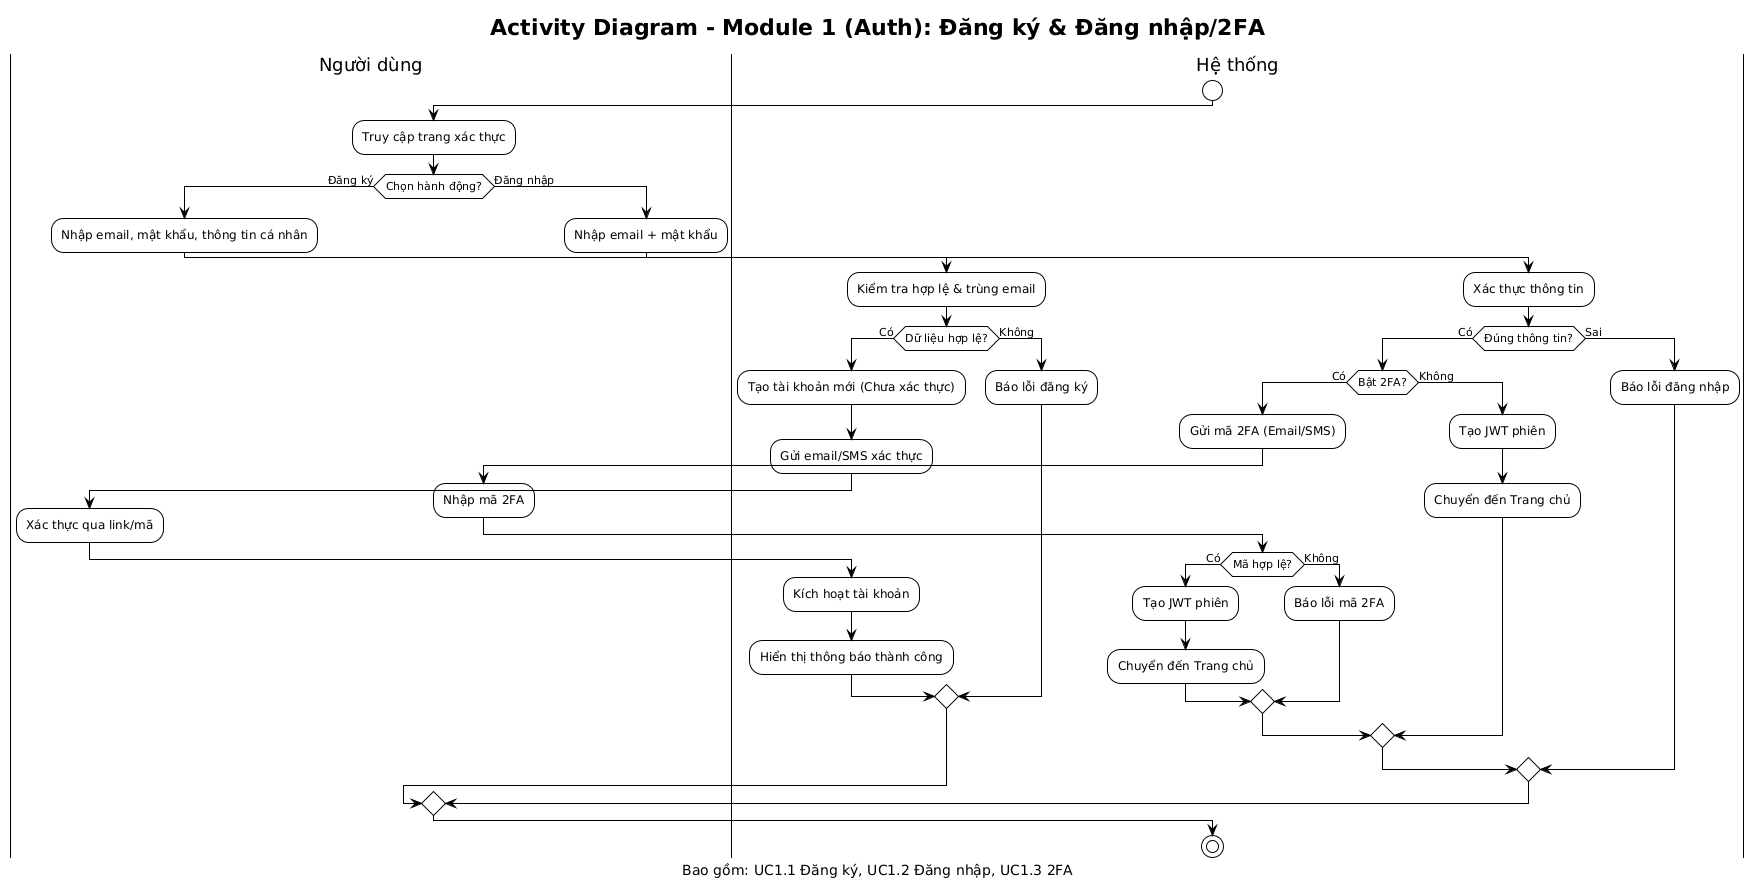
\includegraphics[width=\textwidth]{Images/Activity diagrams/AD-M1-Auth-Register-Login.png}
  \caption{Activity Diagram - Đăng ký và Đăng nhập (AD-M1-Auth-Register-Login)}
\end{figure}

\subsubsection{AD-M1-Auth-Recovery-Logout}

Diagram này mô tả quy trình khôi phục mật khẩu và đăng xuất của người dùng.

\textbf{UC1.4 – Khôi phục mật khẩu:} Người dùng nhập email. Hệ thống kiểm tra và gửi link/mã OTP (bảo mật: luôn trả về thông báo chung). Người dùng mở link/nhập mã và đặt mật khẩu mới. Hệ thống xác thực và cập nhật mật khẩu.

\textbf{UC1.5 – Đăng xuất:} Người dùng nhấn "Đăng xuất". Hệ thống hủy phiên, xóa JWT token và blacklist token trên server, sau đó chuyển hướng về Trang chủ.

\begin{figure}[H]
  \centering
  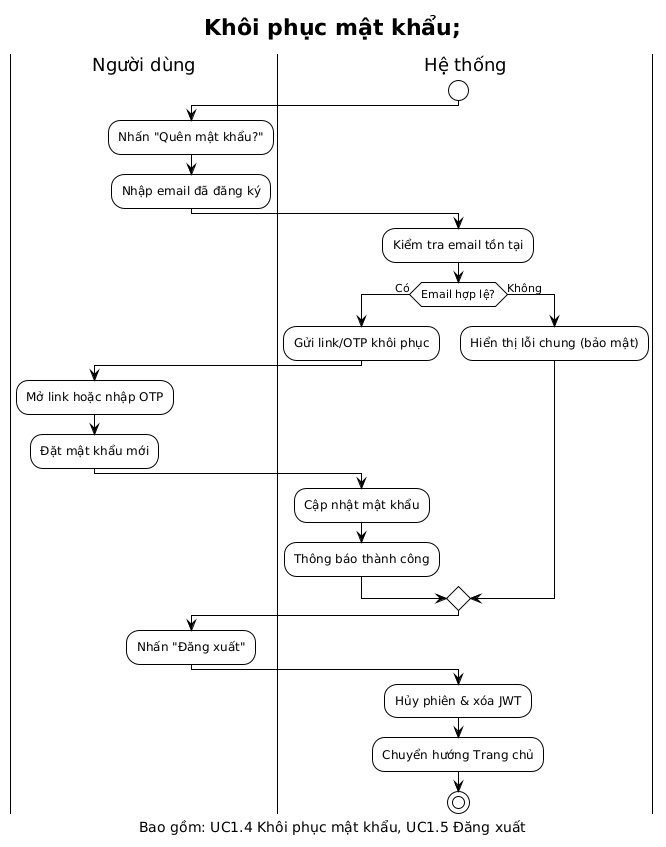
\includegraphics[width=\textwidth]{Images/Activity diagrams/AD-M1-Auth-Recovery-Logout.png}
  \caption{Activity Diagram - Khôi phục mật khẩu và Đăng xuất (AD-M1-Auth-Recovery-Logout)}
\end{figure}

\subsubsection{AD-M1-Profile-EditPrivacy}

Diagram này mô tả quy trình chỉnh sửa hồ sơ cá nhân và cài đặt quyền riêng tư.

\textbf{UC1.6 – Quản lý hồ sơ:} Người dùng cập nhật thông tin (bio, ảnh đại diện, ảnh bìa). Hệ thống upload ảnh (nếu có), xác thực dữ liệu, và cập nhật thông tin trong database. Nếu có lỗi, hệ thống trả về thông báo lỗi cụ thể.

\textbf{UC1.7 – Quyền riêng tư:} Người dùng điều chỉnh cài đặt ai có thể xem hồ sơ, bài đăng và nhắn tin (công khai, chỉ bạn bè, chỉ mình tôi). Hệ thống lưu cấu hình vào database và áp dụng ngay lập tức.

\begin{figure}[H]
  \centering
  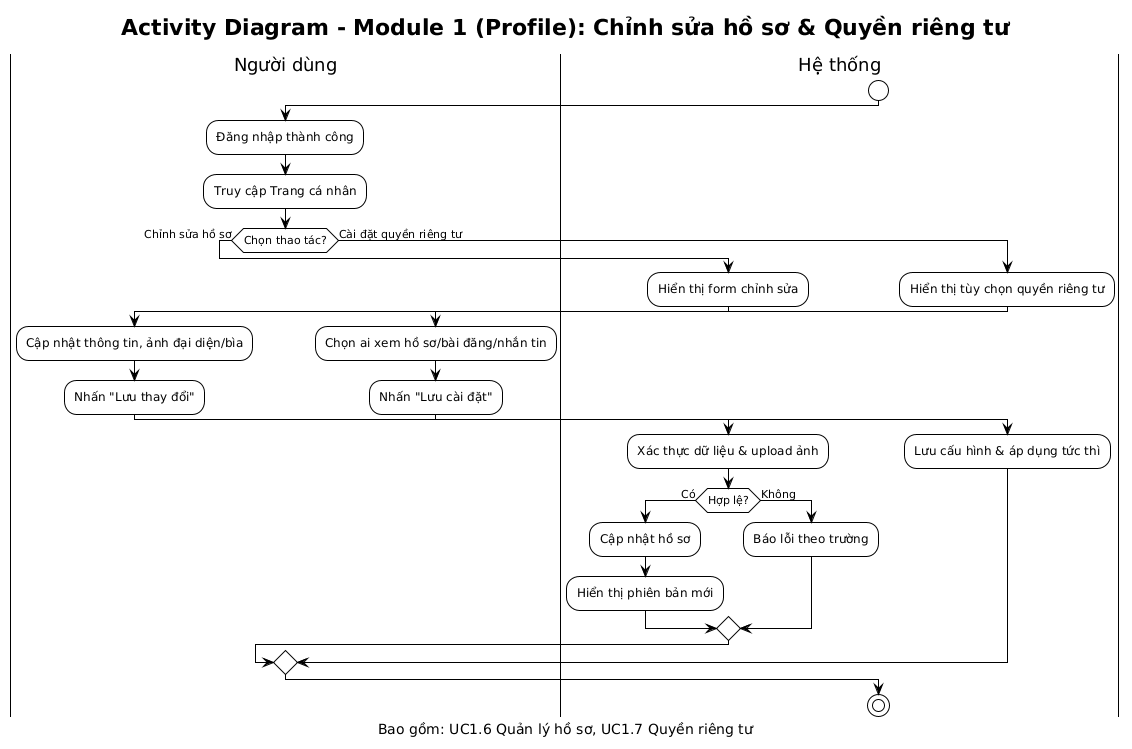
\includegraphics[width=\textwidth]{Images/Activity diagrams/AD-M1-Profile-EditPrivacy.png}
  \caption{Activity Diagram - Chỉnh sửa hồ sơ và Quyền riêng tư (AD-M1-Profile-EditPrivacy)}
\end{figure}

\subsubsection{AD-M1-Profile-SellerUpgrade}

Diagram này mô tả quy trình đăng ký trở thành người bán (Seller).

\textbf{UC1.8 – Đăng ký Người bán:} Buyer điền form đăng ký với thông tin shop (tên shop, địa chỉ, số điện thoại, giấy tờ pháp lý). Hệ thống lưu với trạng thái \textit{pending} và gửi email xác minh. Sau khi xác minh thành công, hệ thống cập nhật trạng thái thành \textit{approved}, thay đổi vai trò từ \textit{buyer} sang \textit{seller}, và chuyển hướng đến Seller Dashboard.

\begin{figure}[H]
  \centering
  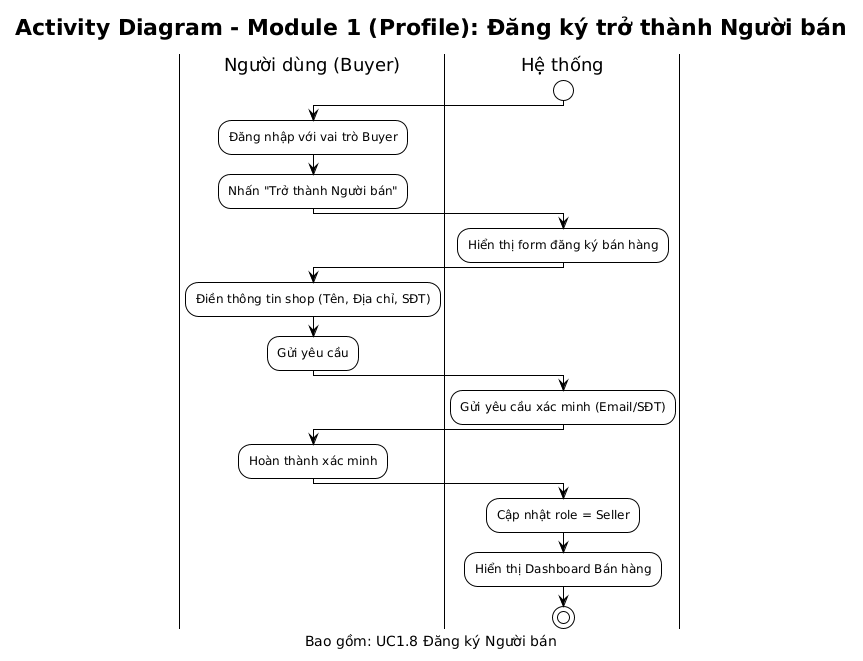
\includegraphics[width=\textwidth]{Images/Activity diagrams/AD-M1-Profile-SellerUpgrade.png}
  \caption{Activity Diagram - Đăng ký trở thành Người bán (AD-M1-Profile-SellerUpgrade)}
\end{figure}

\subsection{Module 2 – Social \& Content}

Module này tập trung vào các tính năng mạng xã hội: xem feed cá nhân hóa, tạo và quản lý bài đăng, tương tác, follow, nhắn tin, tham gia nhóm, và báo cáo vi phạm.

\subsubsection{AD-M2-FeedAndPosts}

Diagram này mô tả quy trình xem feed, tạo bài đăng và tương tác với nội dung.

\textbf{UC2.1 – Xem Feed:} Người dùng truy cập Trang chủ. Hệ thống truy vấn database lấy bài đăng từ người đang theo dõi kết hợp gợi ý, áp dụng thuật toán sắp xếp. Feed hiển thị với tính năng infinite scroll.

\textbf{UC2.2 – Tạo bài đăng:} Người dùng nhập nội dung văn bản và tải hình ảnh (nếu có). Seller có thể gắn thẻ sản phẩm (UC2.3). Hệ thống kiểm tra nội dung, lưu bài đăng vào database, và hiển thị trên feed.

\textbf{UC2.3 – Gắn thẻ sản phẩm:} Seller chọn một hoặc nhiều sản phẩm từ shop để gắn thẻ vào bài đăng. Người dùng xem bài đăng có thể nhấn vào thẻ sản phẩm để chuyển đến trang chi tiết.

\textbf{UC2.4 – Tương tác với bài đăng:} Người dùng có thể thích hoặc bình luận bài đăng. Hệ thống cập nhật số lượt thích/bình luận, lưu vào database và gửi thông báo đến chủ sở hữu bài đăng (UC7.1).

\begin{figure}[H]
  \centering
  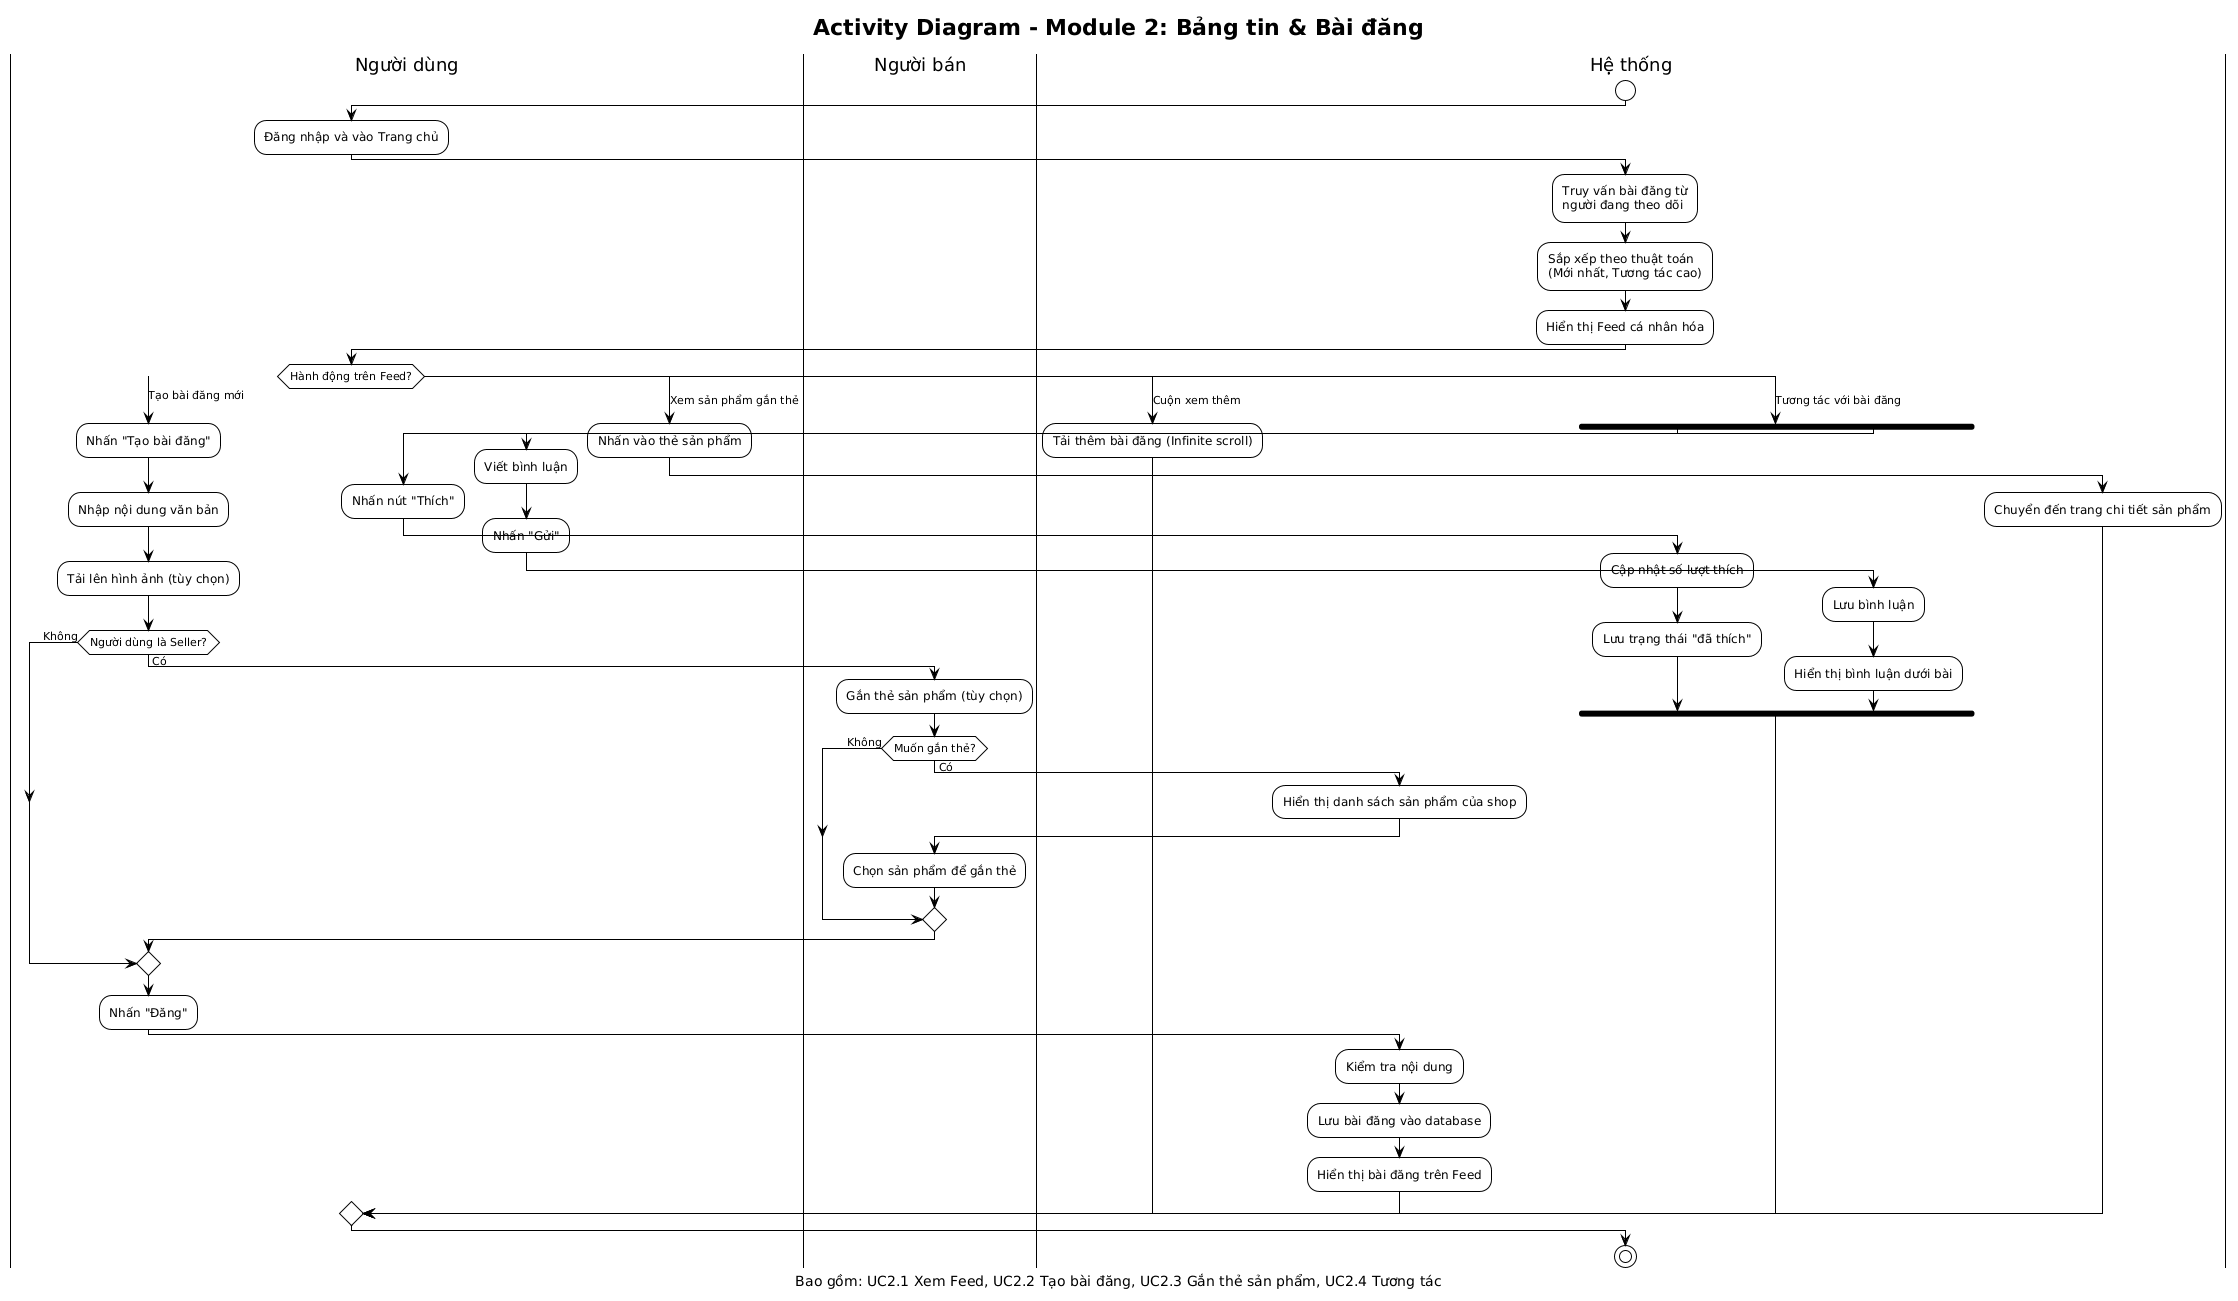
\includegraphics[width=\textwidth]{Images/Activity diagrams/AD-M2-FeedAndPosts.png}
  \caption{Activity Diagram - Feed và Bài đăng (AD-M2-FeedAndPosts)}
\end{figure}

\subsubsection{AD-M2-SocialConnections}

Diagram này mô tả các kết nối xã hội giữa người dùng, bao gồm follow, nhắn tin, tham gia nhóm và báo cáo vi phạm.

\textbf{UC2.5 – Theo dõi người dùng:} Người dùng A nhấn "Theo dõi" trên trang cá nhân của B. Hệ thống tạo mối quan hệ follow, cập nhật số người theo dõi, gửi thông báo đến B, và bài đăng của B sẽ xuất hiện trên Feed của A.

\textbf{UC2.6 – Nhắn tin 1-1:} Người dùng A gửi tin nhắn cho B. Hệ thống kiểm tra B có chặn A hay không. Nếu không bị chặn, hệ thống lưu tin nhắn vào database và gửi real-time đến B qua WebSocket (Socket.io).

\textbf{UC2.7 – Tham gia nhóm:} Người dùng A chọn nhóm và nhấn "Tham gia". Nếu là nhóm công khai, hệ thống thêm A vào nhóm ngay lập tức. Nếu là nhóm riêng tư, hệ thống gửi yêu cầu và chờ Admin phê duyệt.

\textbf{UC2.8 – Báo cáo vi phạm:} Người dùng A chọn đối tượng báo cáo (bài đăng, bình luận hoặc người dùng), chọn lý do vi phạm và thêm mô tả (nếu có). Hệ thống lưu báo cáo với trạng thái \textit{pending}, thông báo Admin và hiển thị "Báo cáo đã được ghi nhận".

\begin{figure}[H]
  \centering
  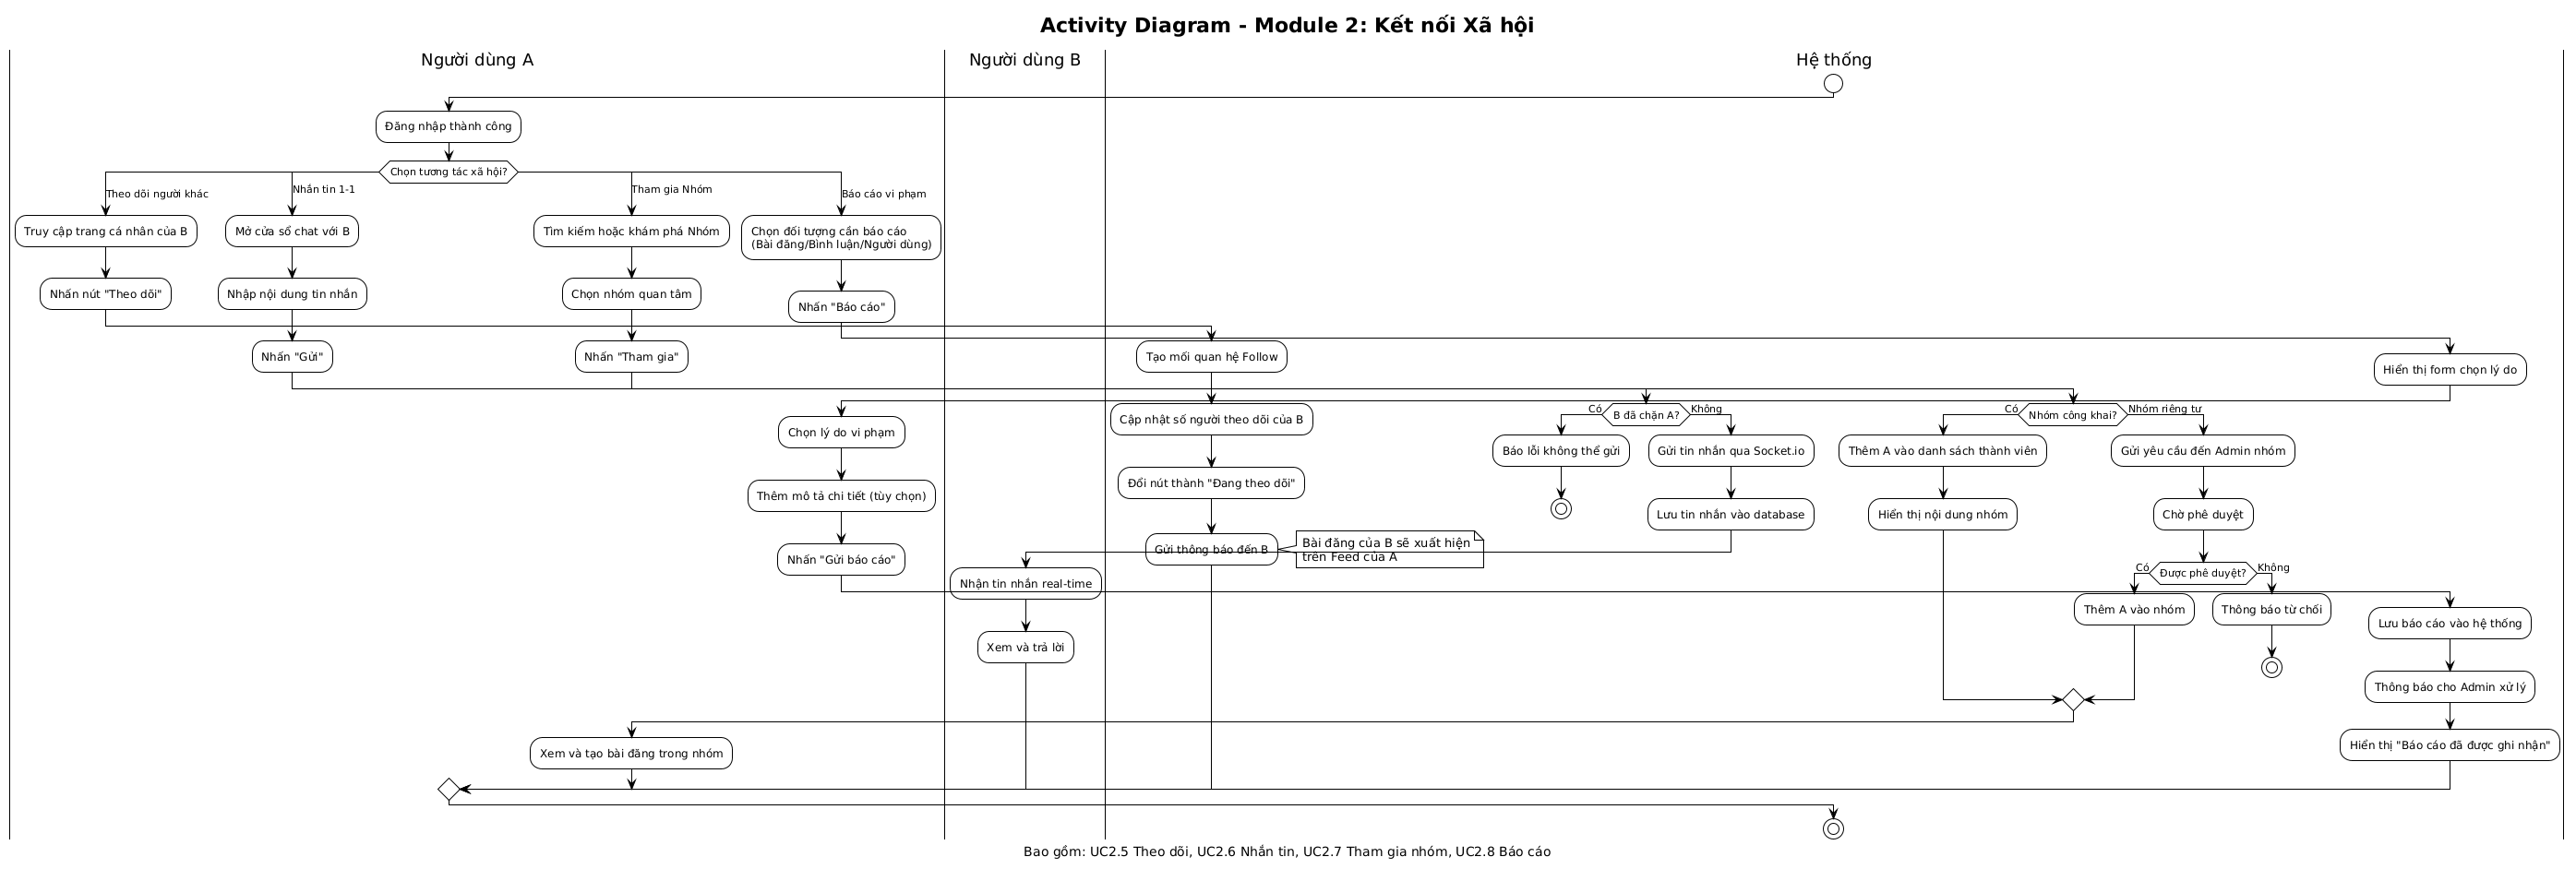
\includegraphics[width=\textwidth]{Images/Activity diagrams/AD-M2-SocialConnections.png}
  \caption{Activity Diagram - Kết nối Xã hội (AD-M2-SocialConnections)}
\end{figure}

\subsection{Module 3 – Commerce}

Module này bao quát hệ sinh thái thương mại điện tử: hành trình mua hàng của Buyer (tìm kiếm, xem sản phẩm, giỏ hàng, thanh toán, theo dõi đơn hàng, đánh giá) và quản lý của Seller (sản phẩm, đơn hàng, hoàn tiền, phản hồi đánh giá).

\subsubsection{AD-M3-BuyerFlow}

Diagram này mô tả toàn bộ quy trình mua hàng từ góc nhìn của người mua (Buyer).

\textbf{UC3.1 – Tìm kiếm và lọc sản phẩm:} Buyer nhập từ khóa và áp dụng bộ lọc (danh mục, khoảng giá, tags). Hệ thống truy vấn database và hiển thị danh sách sản phẩm phù hợp hoặc thông báo không tìm thấy.

\textbf{UC3.2 – Xem chi tiết sản phẩm và chọn biến thể:} Buyer chọn sản phẩm, hệ thống hiển thị chi tiết (hình ảnh, mô tả, giá, tồn kho, đánh giá). Buyer chọn biến thể (size, màu) và số lượng.

\textbf{UC3.3 – Thêm vào giỏ hàng:} Buyer nhấn "Thêm vào giỏ hàng". Hệ thống kiểm tra tồn kho, nếu còn hàng thì lưu vào giỏ hàng và cập nhật số lượng. Nếu hết hàng, hệ thống trả về lỗi và đề xuất sản phẩm tương tự.

\textbf{UC3.4 – Quản lý giỏ hàng:} Buyer truy cập giỏ hàng, hệ thống hiển thị danh sách sản phẩm và tổng tiền. Buyer có thể cập nhật số lượng hoặc xóa sản phẩm, hệ thống tự động tính lại tổng tiền.

\textbf{UC3.5 – Thanh toán:} Buyer nhấn "Thanh toán". Hệ thống kiểm tra tồn kho lần cuối. Nếu đủ hàng, Buyer nhập địa chỉ giao hàng và chọn phương thức thanh toán. Hệ thống tạo đơn hàng với trạng thái \textit{Processing}, làm rỗng giỏ hàng, gửi thông báo cho Seller và hiển thị "Đặt hàng thành công".

\textbf{UC3.6 – Theo dõi đơn hàng:} Buyer xem "Đơn hàng của tôi", hệ thống hiển thị danh sách đơn hàng với mã, trạng thái và ngày đặt. Buyer có thể xem chi tiết và theo dõi trạng thái real-time.

\textbf{UC3.7 – Đánh giá sản phẩm:} Khi đơn hàng đã giao (\textit{Delivered}), Buyer có thể đánh giá sản phẩm (chọn số sao, viết nhận xét, tải ảnh). Hệ thống lưu đánh giá và hiển thị trên trang chi tiết sản phẩm.

\begin{figure}[H]
  \centering
  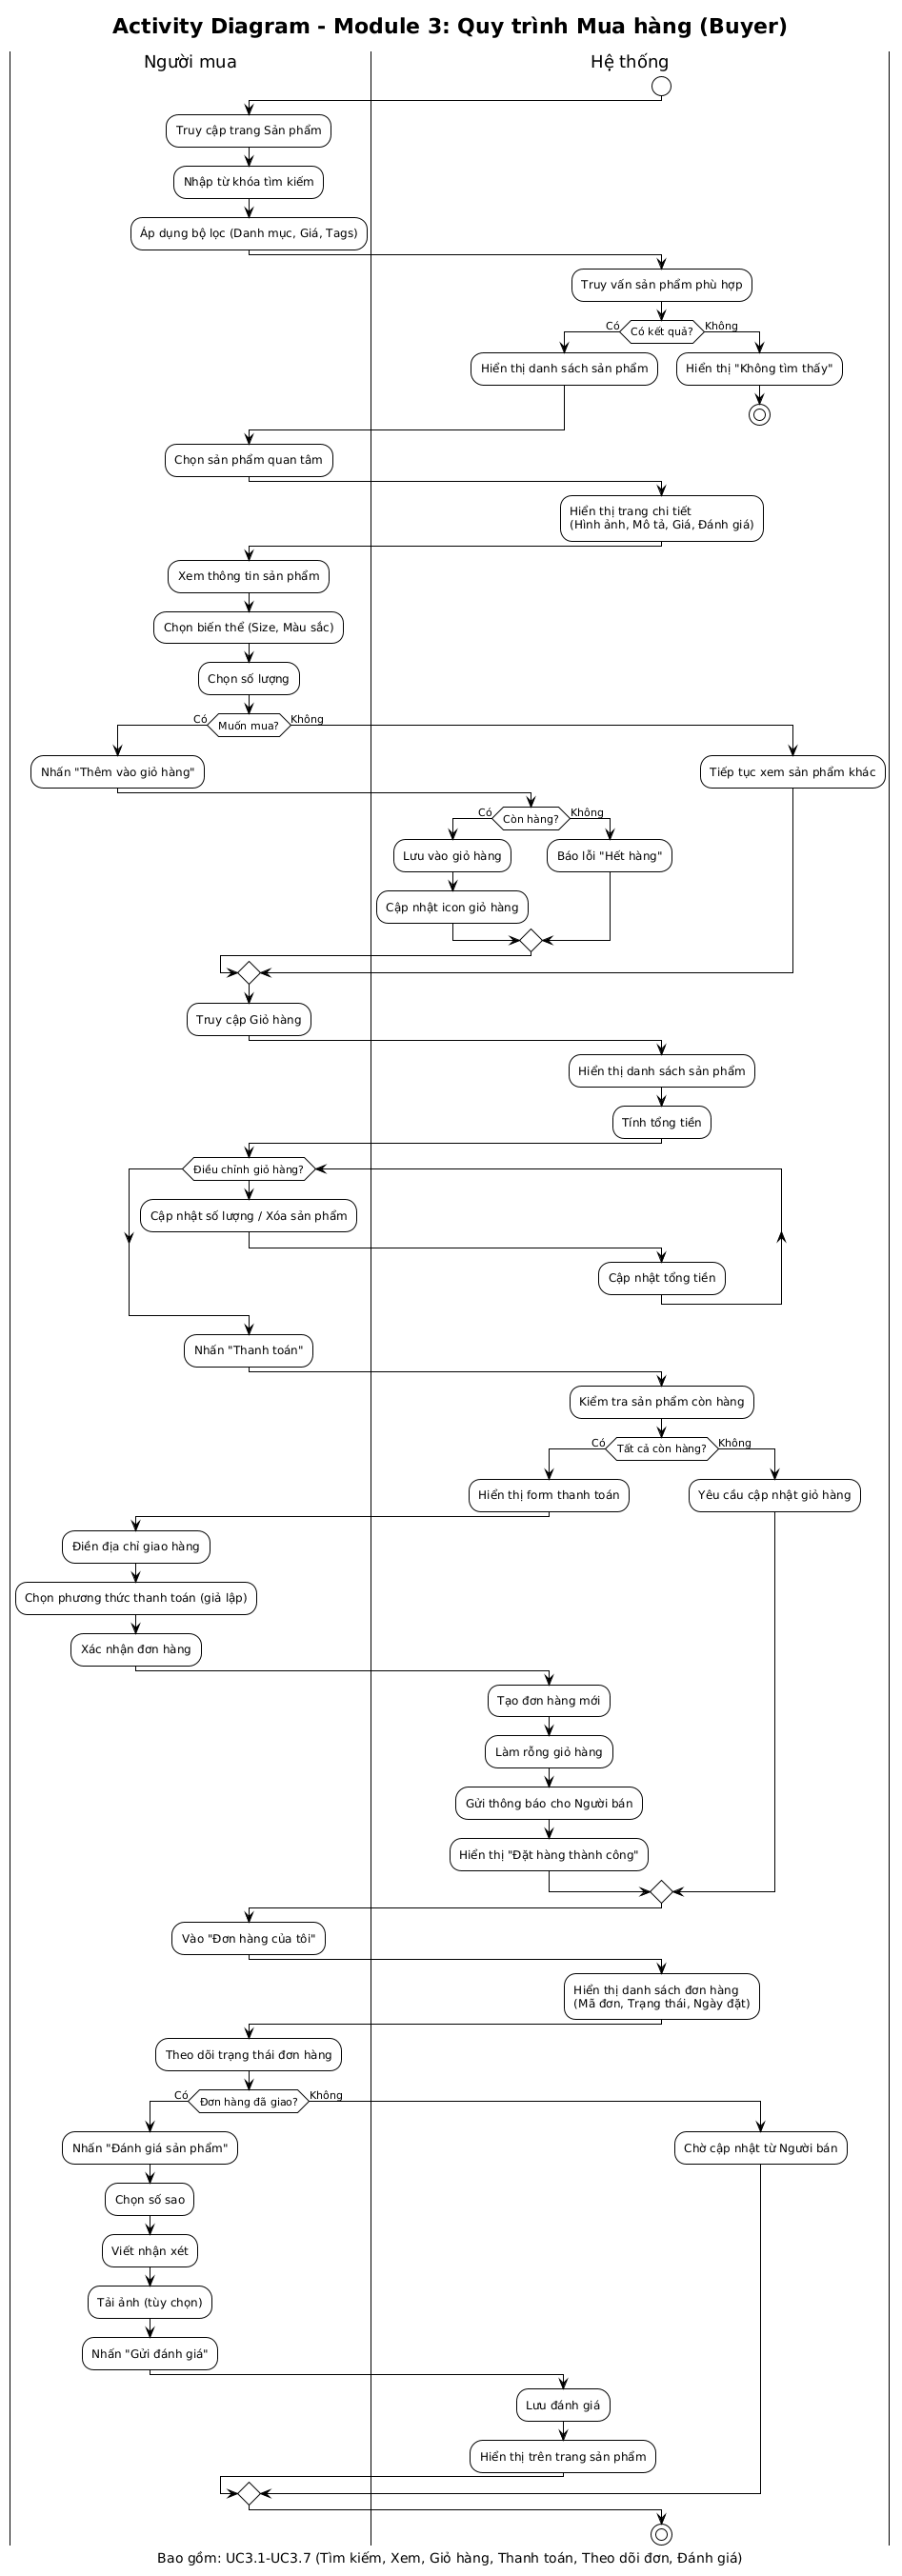
\includegraphics[width=\textwidth]{Images/Activity diagrams/AD-M3-BuyerFlow.png}
  \caption{Activity Diagram - Quy trình Mua hàng (AD-M3-BuyerFlow)}
\end{figure}

\subsubsection{AD-M3-Seller-ProductsOrders}

Diagram này mô tả các tác vụ quản lý sản phẩm và đơn hàng của Seller.

\textbf{UC3.8 – Quản lý sản phẩm:} Seller truy cập Dashboard Bán hàng, chọn "Quản lý Sản phẩm". Seller có thể thêm (tên, mô tả, giá, tồn kho, hình ảnh, biến thể), sửa hoặc xóa sản phẩm (soft delete). Hệ thống xác thực và lưu vào database.

\textbf{UC3.10 – Quản lý đơn hàng:} Seller chọn "Quản lý Đơn hàng", hệ thống hiển thị danh sách đơn hàng. Seller xem chi tiết và cập nhật trạng thái: "Đang xử lý", "Đang giao", "Đã giao", hoặc "Đã hủy". Hệ thống lưu thay đổi, ghi lịch sử và gửi thông báo đến Buyer.

\begin{figure}[H]
  \centering
  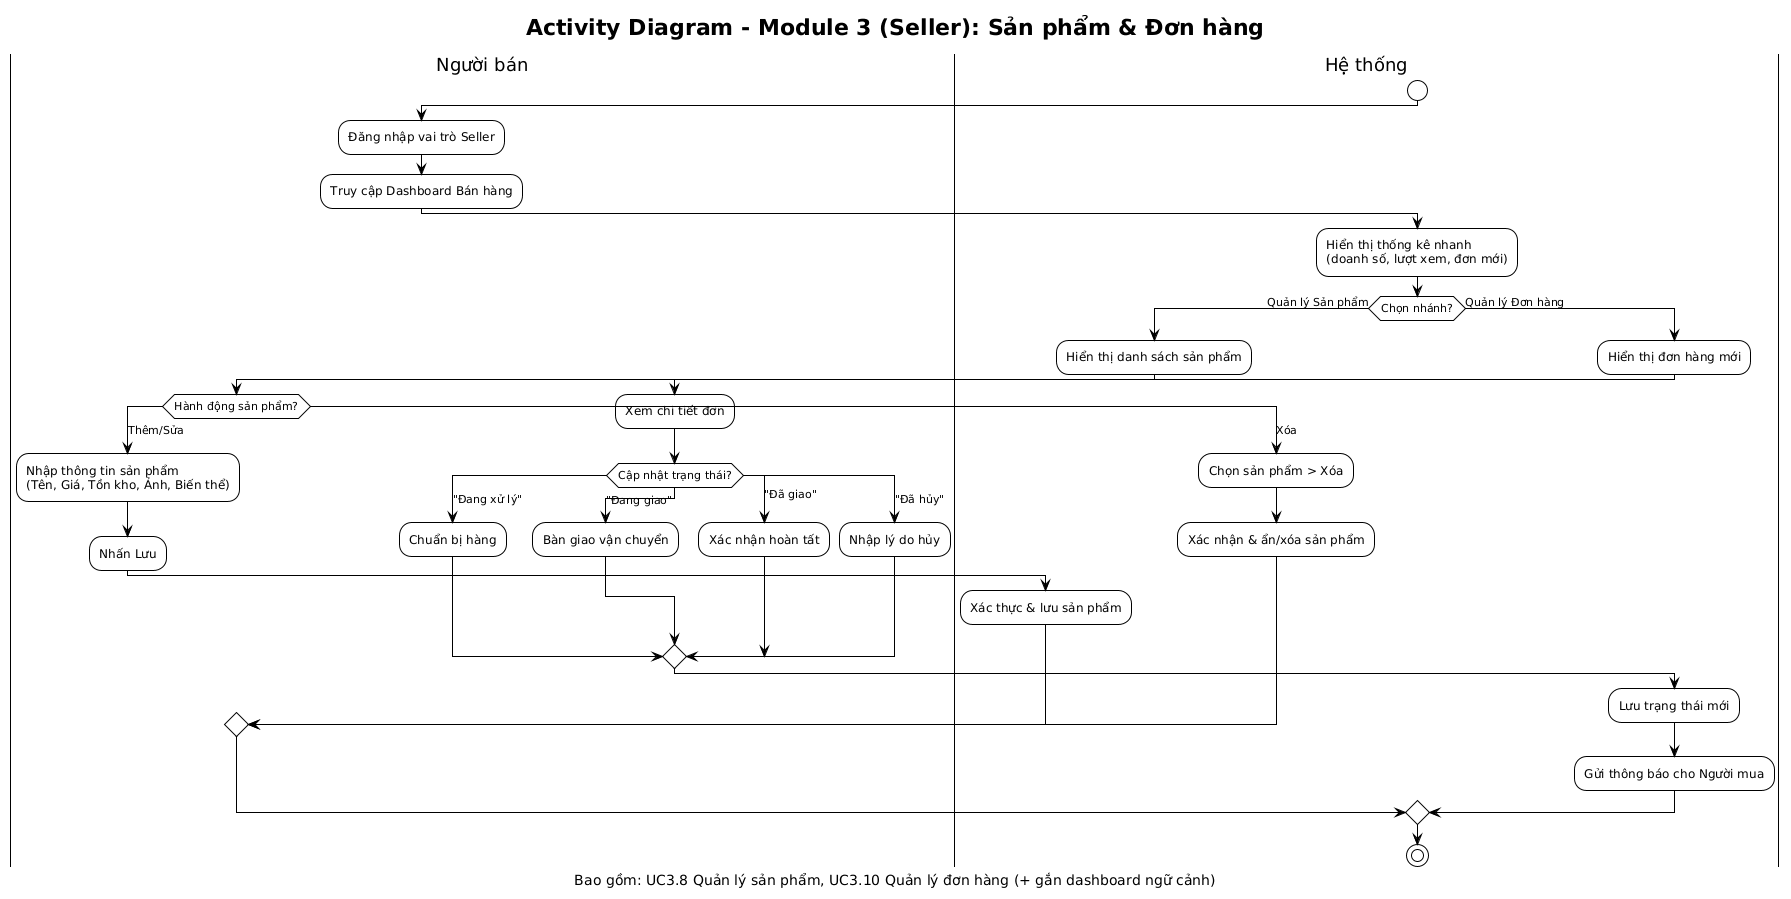
\includegraphics[width=\textwidth]{Images/Activity diagrams/AD-M3-Seller-ProductsOrders.png}
  \caption{Activity Diagram - Quản lý Sản phẩm và Đơn hàng của Seller (AD-M3-Seller-ProductsOrders)}
\end{figure}

\subsubsection{AD-M3-Seller-RefundReview}

Diagram này mô tả quy trình xử lý hoàn tiền và phản hồi đánh giá của Seller.

\textbf{UC3.11 – Xử lý hoàn tiền:} Seller chọn "Xử lý hoàn tiền", hệ thống hiển thị danh sách yêu cầu hoàn tiền. Seller xem chi tiết và quyết định chấp nhận hoặc từ chối. Nếu chấp nhận, hệ thống cập nhật trạng thái \textit{Refunded}, xử lý hoàn tiền và gửi thông báo. Nếu từ chối, hệ thống lưu lý do và gửi thông báo đến Buyer.

\textbf{UC3.12 – Phản hồi đánh giá:} Seller chọn "Đánh giá", hệ thống hiển thị danh sách đánh giá từ Buyer. Seller chọn đánh giá cần phản hồi, nhập nội dung và gửi. Hệ thống lưu phản hồi và hiển thị dưới đánh giá gốc trên trang sản phẩm.

\begin{figure}[H]
  \centering
  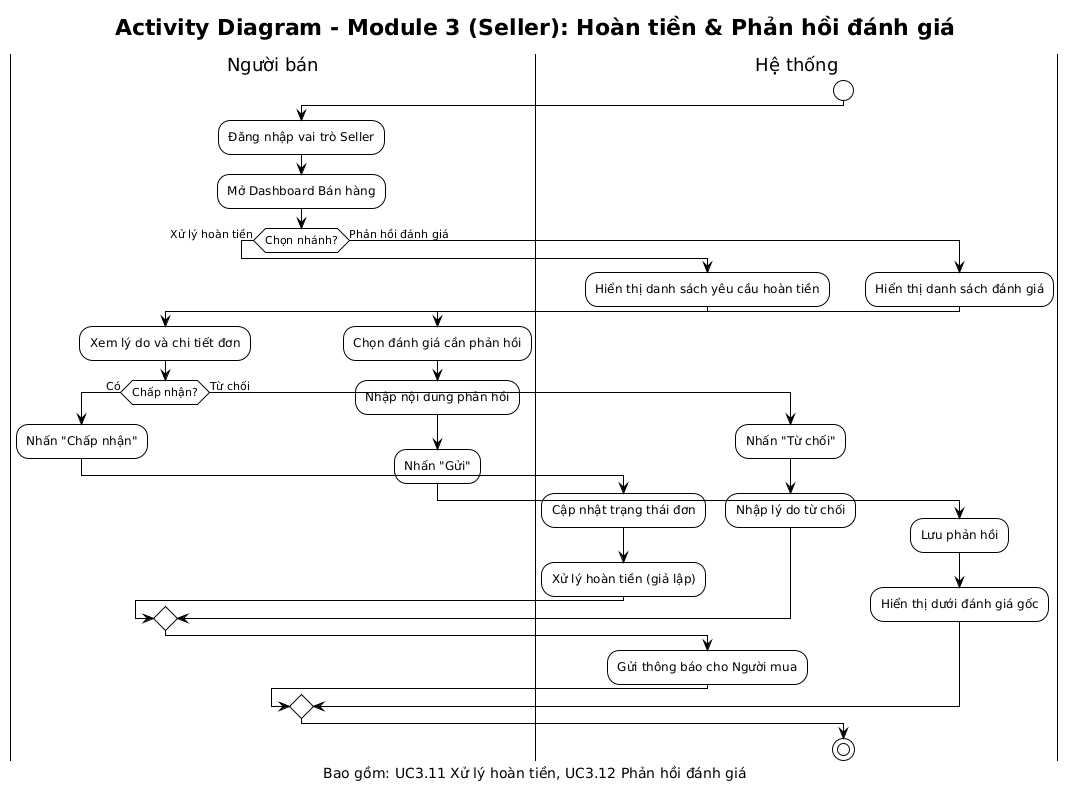
\includegraphics[width=\textwidth]{Images/Activity diagrams/AD-M3-Seller-RefundReview.png}
  \caption{Activity Diagram - Hoàn tiền và Phản hồi Đánh giá của Seller (AD-M3-Seller-RefundReview)}
\end{figure}

\subsection{Module 4 – Admin}

Module này cung cấp công cụ quản trị: quản lý tài khoản (vô hiệu hóa, kích hoạt, thay đổi vai trò), quản lý nội dung (duyệt và xóa bài đăng, sản phẩm vi phạm), xử lý báo cáo vi phạm, và thống kê tổng quan hệ thống.

\subsubsection{AD-M4-Admin-AccountsContent}

Diagram này mô tả quy trình quản lý tài khoản người dùng và nội dung của Admin.

\textbf{UC4.1 – Quản lý tài khoản:} Admin chọn "Quản lý Tài khoản", hệ thống hiển thị danh sách người dùng. Admin có thể tìm kiếm/lọc theo tên, email, vai trò, trạng thái. Admin có thể vô hiệu hóa, kích hoạt lại, hoặc đổi vai trò người dùng. Mỗi hành động được ghi lịch sử và cập nhật database.

\textbf{UC4.2 – Quản lý nội dung:} Admin chọn "Quản lý Nội dung", hệ thống hiển thị danh sách bài đăng và sản phẩm (có thể lọc theo loại, người đăng, trạng thái). Admin xem chi tiết và có thể xóa nội dung vi phạm. Hệ thống xóa/ẩn nội dung và gửi email thông báo đến chủ sở hữu.

\begin{figure}[H]
  \centering
  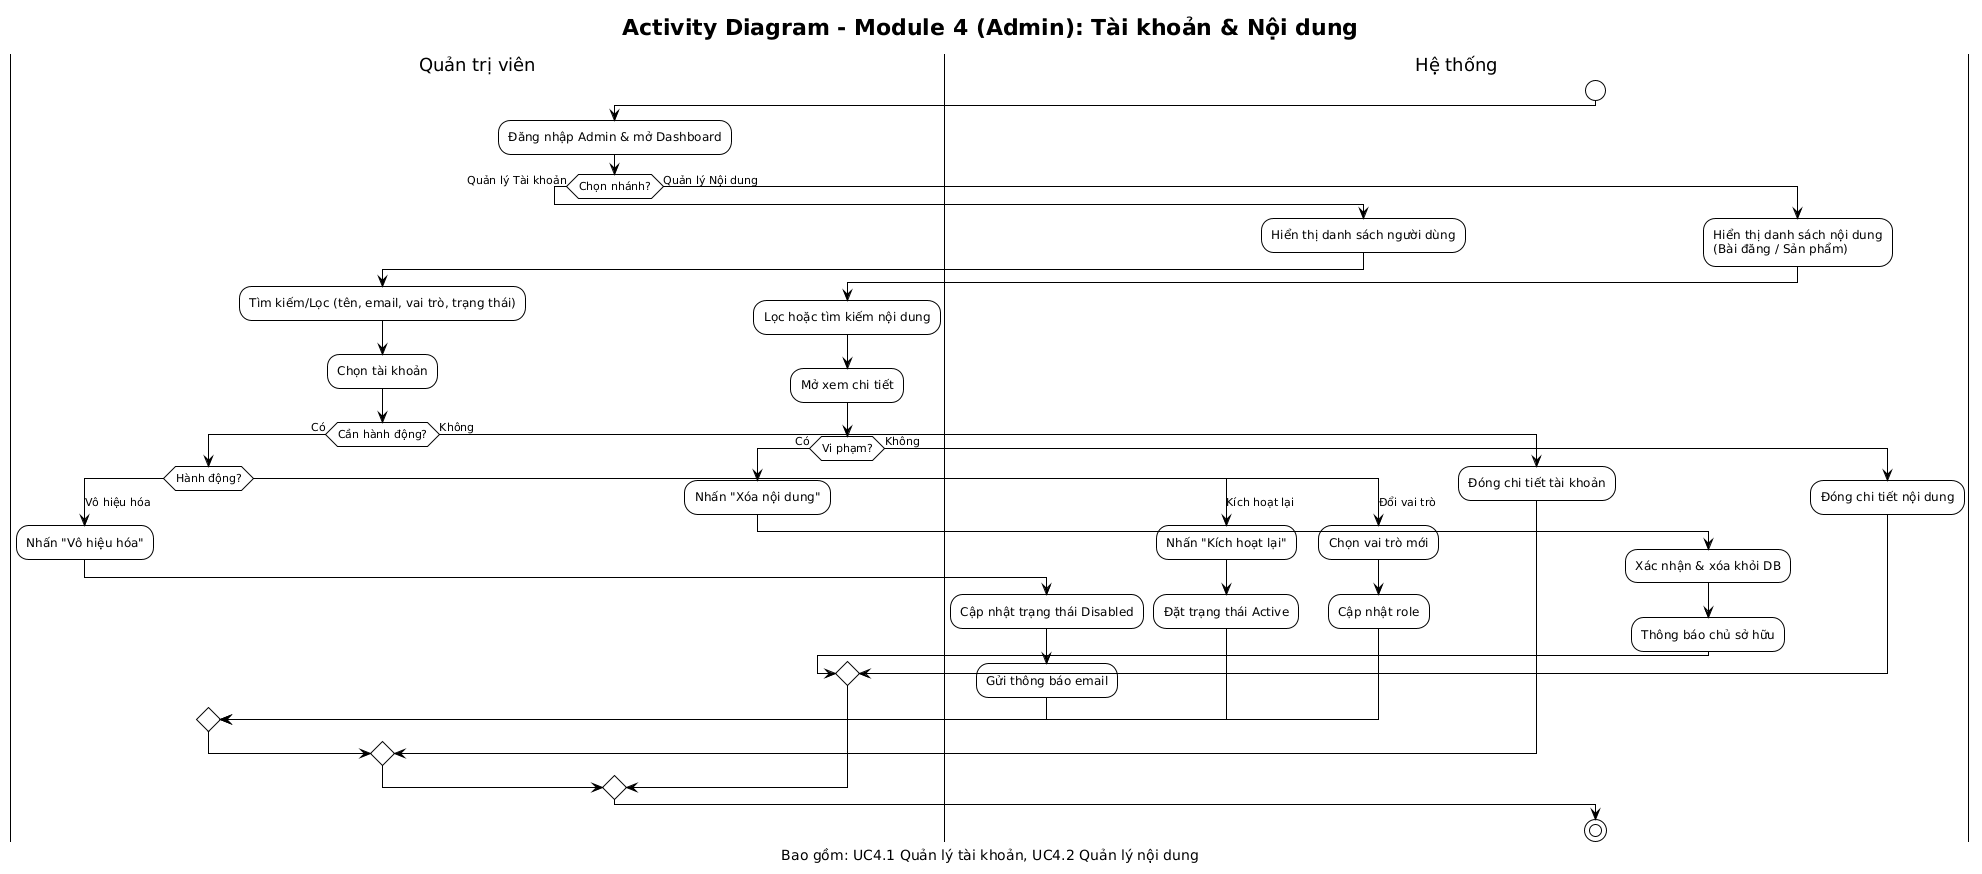
\includegraphics[width=\textwidth]{Images/Activity diagrams/AD-M4-Admin-AccountsContent.png}
  \caption{Activity Diagram - Quản lý Tài khoản và Nội dung của Admin (AD-M4-Admin-AccountsContent)}
\end{figure}

\subsubsection{AD-M4-Admin-ReportsAnalytics}

Diagram này mô tả quy trình xử lý báo cáo vi phạm và xem thống kê phân tích của Admin.

\textbf{UC4.3 – Xử lý báo cáo vi phạm:} Admin chọn "Xử lý báo cáo vi phạm", hệ thống hiển thị danh sách báo cáo đang chờ (sắp xếp theo mức độ ưu tiên). Admin xem chi tiết và đánh giá tính hợp lệ. Nếu hợp lệ, Admin chọn hành động: xóa nội dung, khóa tài khoản, hoặc gửi cảnh cáo. Hệ thống thực thi hành động, đánh dấu "Đã xử lý" và gửi thông báo. Nếu không hợp lệ, Admin đánh dấu "Từ chối".

\textbf{UC4.4 – Thống kê và phân tích:} Admin chọn khoảng thời gian và xem Dashboard với các chỉ số: số lượng người dùng (mới, tổng), tỷ lệ Buyer/Seller, số lượng bài đăng/sản phẩm mới, hoạt động giao dịch (đơn hàng, doanh thu). Dashboard có biểu đồ trực quan hóa xu hướng theo thời gian.

\begin{figure}[H]
  \centering
  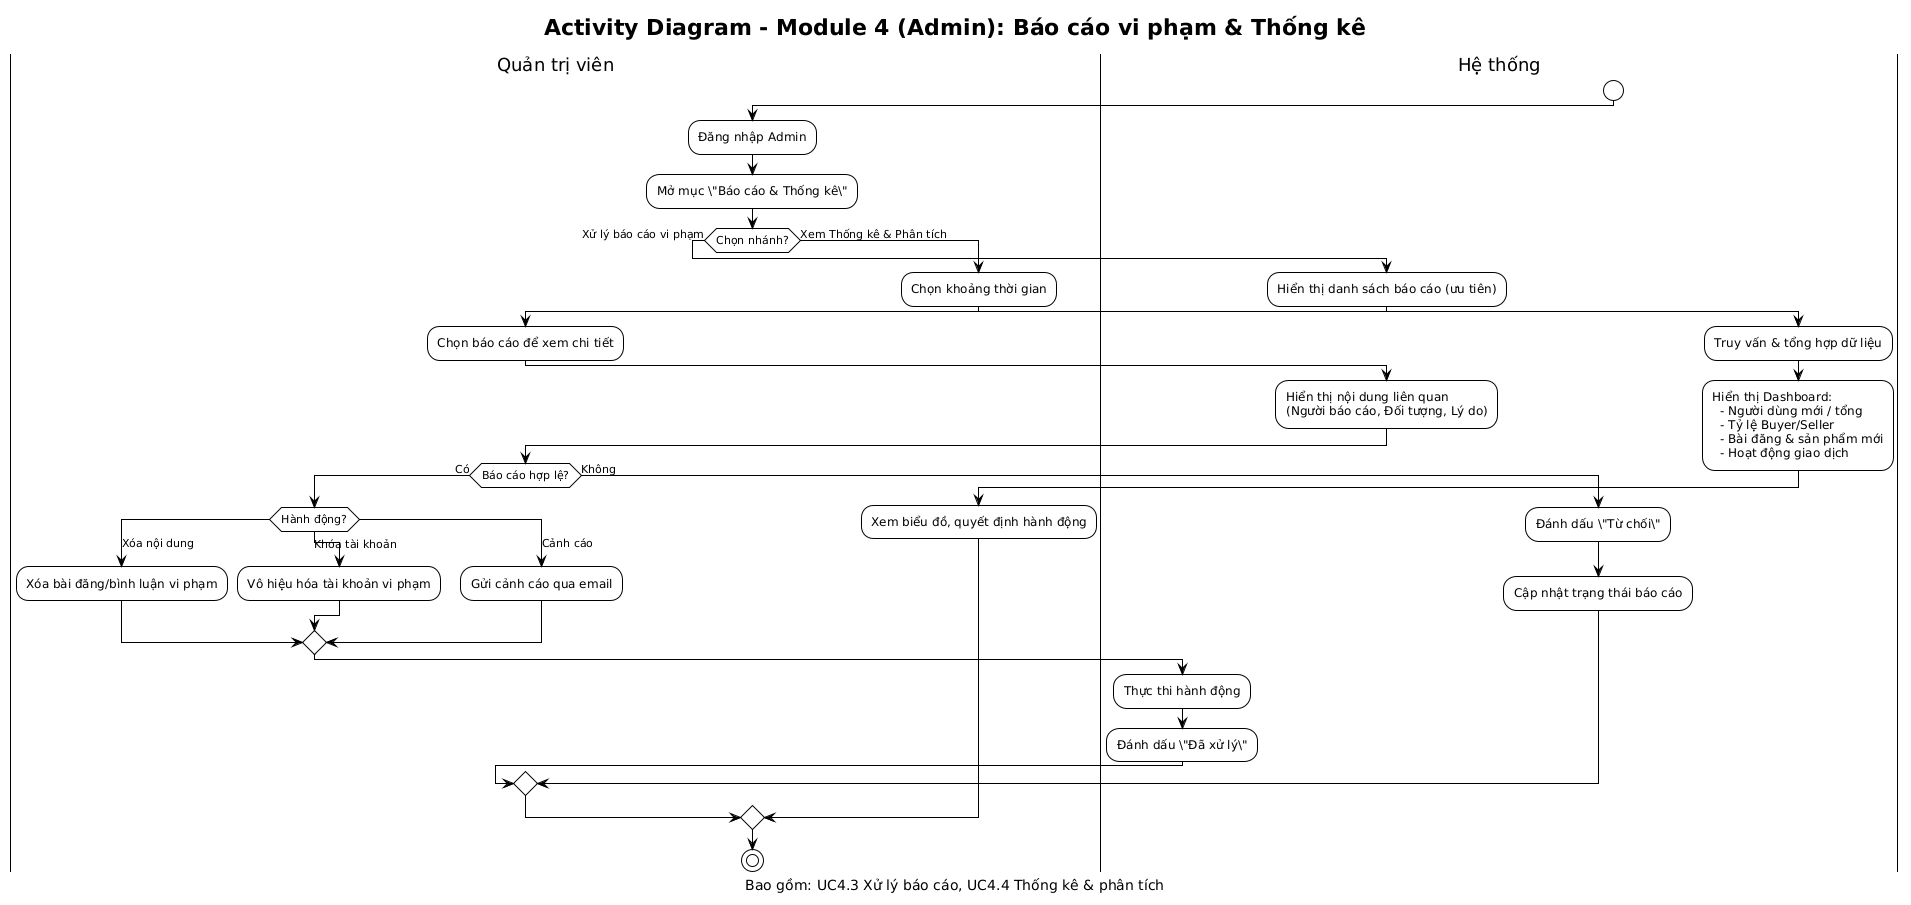
\includegraphics[width=\textwidth]{Images/Activity diagrams/AD-M4-Admin-ReportsAnalytics.png}
  \caption{Activity Diagram - Báo cáo và Thống kê của Admin (AD-M4-Admin-ReportsAnalytics)}
\end{figure}

\subsection{Module 5 – AI Content Assistant}

Module này tích hợp AI (Google Gemini API) để hỗ trợ tạo nội dung đa phương thức: generate text, generate image+text, và generate video+images+text. Luồng xử lý được thiết kế theo mô hình \textbf{Evaluate--Refine Loop}: sau khi gọi API tạo nội dung, hệ thống tự động đánh giá chất lượng kết quả dựa trên các tiêu chí đã định nghĩa. Nếu điểm đánh giá chưa đạt ngưỡng ($< 7.0/10$), hệ thống phân tích tiêu chí yếu, bổ sung ràng buộc vào prompt và gọi lại API (tối đa 3 lần). Kết quả tốt nhất được trả về cho người dùng kèm điểm đánh giá chi tiết và gợi ý chỉnh sửa.

\subsubsection{AD-M5-UC5.1-GenerateText}

Diagram này mô tả quy trình tạo nội dung bài đăng từ mô tả, ý tưởng và hình ảnh sản phẩm sử dụng Google Gemini API, bao gồm vòng lặp đánh giá và cải thiện tự động.

\textbf{UC5.1 – Tạo bài viết từ mô tả, ý tưởng và hình ảnh sản phẩm:} Người dùng nhập mô tả/ý tưởng và tải hình ảnh sản phẩm (nếu có), nhấn ``Tạo bài viết với AI''. Hệ thống thực hiện quy trình sau:

\begin{enumerate}
    \item \textbf{Phân tích đầu vào}: Trích xuất thực thể chính (tên sản phẩm, đặc điểm, lợi ích), xác định giọng điệu và phân loại loại nội dung (quảng cáo, chia sẻ, giáo dục). Nếu có hình ảnh, sử dụng Gemini Vision phân tích nội dung hình.
    \item \textbf{Xây dựng Prompt}: Tổng hợp thông tin vào prompt có cấu trúc 5 phần (System Instruction, Context, User Input, Constraints, Output Format). Ràng buộc bao gồm: độ dài 100--300 từ, 5--10 hashtag, phải có Call-to-Action, output dạng JSON.
    \item \textbf{Gọi API}: Gửi prompt đến Google Gemini API.
    \item \textbf{Đánh giá chất lượng}: Kết quả được chấm điểm theo 6 tiêu chí: Tính liên quan (0.25), Tính hấp dẫn (0.20), Cấu trúc hoàn chỉnh (0.15), Độ dài phù hợp (0.10), Chất lượng ngôn ngữ (0.15), Giá trị thương mại (0.15). Điểm tổng hợp là trung bình có trọng số.
    \item \textbf{Quyết định}: Nếu điểm $\geq$ 7.0 $\rightarrow$ trả kết quả. Nếu $<$ 7.0 và chưa đạt giới hạn 3 lần thử $\rightarrow$ xác định tiêu chí yếu, bổ sung ràng buộc vào prompt, gọi lại API. Nếu đã hết lần thử $\rightarrow$ trả kết quả tốt nhất kèm gợi ý chỉnh sửa.
    \item \textbf{Hiển thị}: Bài viết được chèn vào trình soạn thảo kèm điểm đánh giá chi tiết. Người dùng có thể chỉnh sửa trực tiếp, yêu cầu viết lại đoạn cụ thể, thay đổi giọng điệu, hoặc tạo lại toàn bộ.
\end{enumerate}

\begin{figure}[H]
  \centering
  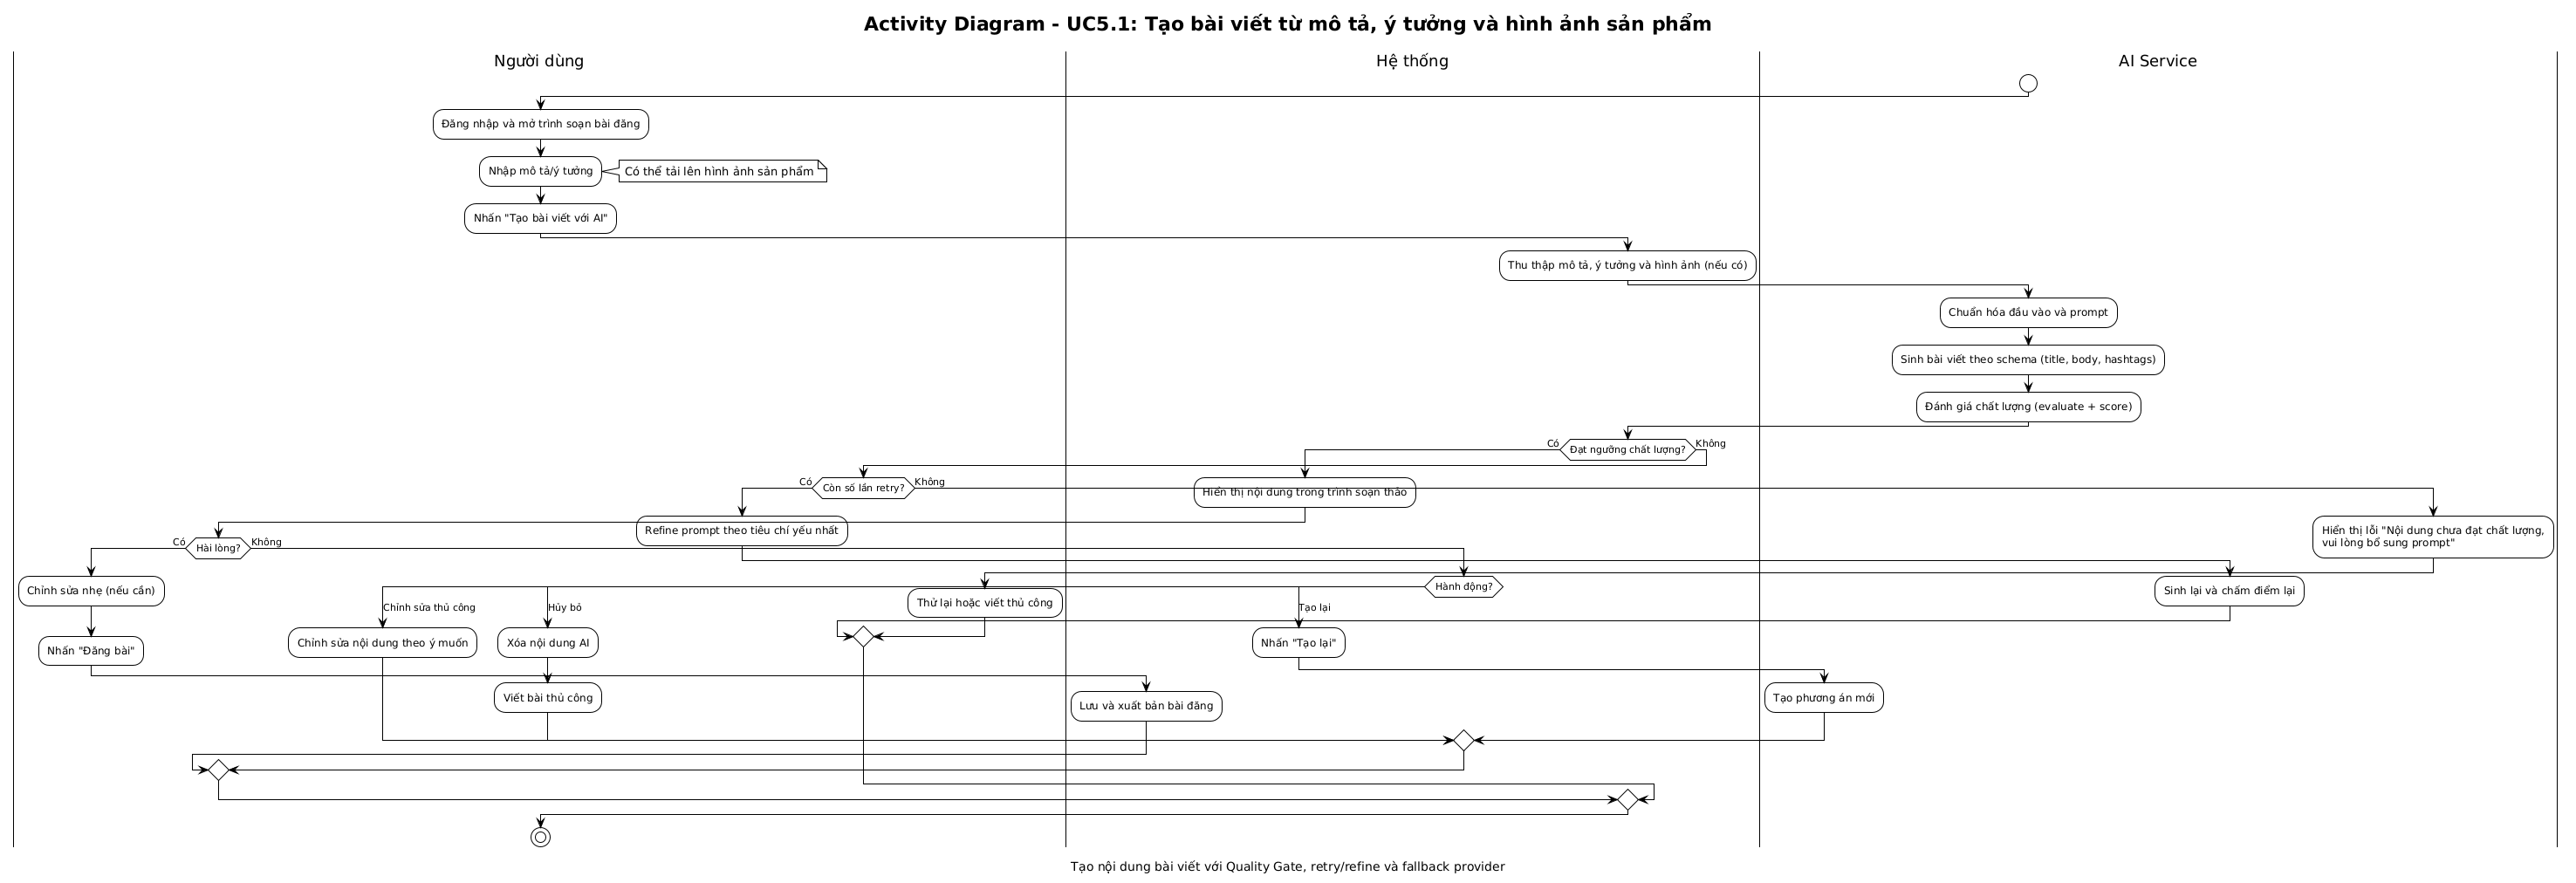
\includegraphics[width=\textwidth]{Images/Activity diagrams/AD-M5-UC5.1-GenerateText.png}
  \caption{Activity Diagram - Tạo bài viết với vòng lặp đánh giá và cải thiện (AD-M5-UC5.1-GenerateText)}
\end{figure}

\subsubsection{AD-M5-UC5.2-GenerateImageText}

Diagram này mô tả quy trình tạo bài viết và hình ảnh từ mô tả, ý tưởng và hình ảnh đầu vào sử dụng Google Gemini API, với đánh giá chất lượng riêng biệt cho text và image.

\textbf{UC5.2 – Tạo bài viết và hình ảnh:} Người dùng nhập mô tả/ý tưởng và hình ảnh đầu vào (nếu có), nhấn ``Tạo bài viết và hình ảnh với AI''. Hệ thống thực hiện quy trình sau:

\begin{enumerate}
    \item \textbf{Phân tích đầu vào}: Tương tự UC5.1, bổ sung phân tích hình ảnh đầu vào để xác định phong cách hình ảnh (màu sắc chủ đạo, bố cục, đối tượng).
    \item \textbf{Xây dựng Prompt kép}: Tạo prompt cho text (tương tự UC5.1) và prompt riêng cho image (bao gồm Visual Spec, phong cách, tỷ lệ 1:1 hoặc 4:5, negative prompt). Nội dung text vừa tạo được dùng làm context cho prompt image.
    \item \textbf{Gọi API}: Gửi prompt text đến Gemini API, sau đó sử dụng kết quả text làm context gửi prompt image.
    \item \textbf{Đánh giá chất lượng}: Text được đánh giá theo 6 tiêu chí (như UC5.1). Image được đánh giá theo 4 tiêu chí riêng: Tính liên quan (0.30), Chất lượng kỹ thuật (0.25), Tính thẩm mỹ (0.25), Nhất quán thương hiệu (0.20). Cả hai phải đạt ngưỡng $\geq$ 7.0/10.
    \item \textbf{Quyết định}: Nếu cả text và image đạt $\rightarrow$ trả kết quả. Nếu chỉ một phần chưa đạt $\rightarrow$ chỉ sửa prompt và tạo lại phần chưa đạt (không cần tạo lại phần đã tốt). Nếu hết lần thử $\rightarrow$ trả kết quả tốt nhất.
    \item \textbf{Hiển thị}: Bài viết và hình ảnh được hiển thị trong trình soạn thảo kèm điểm đánh giá từng loại. Người dùng có thể chỉnh sửa text, tạo lại hình ảnh với phong cách khác, hoặc tải lên hình ảnh thay thế.
\end{enumerate}

\begin{figure}[H]
  \centering
  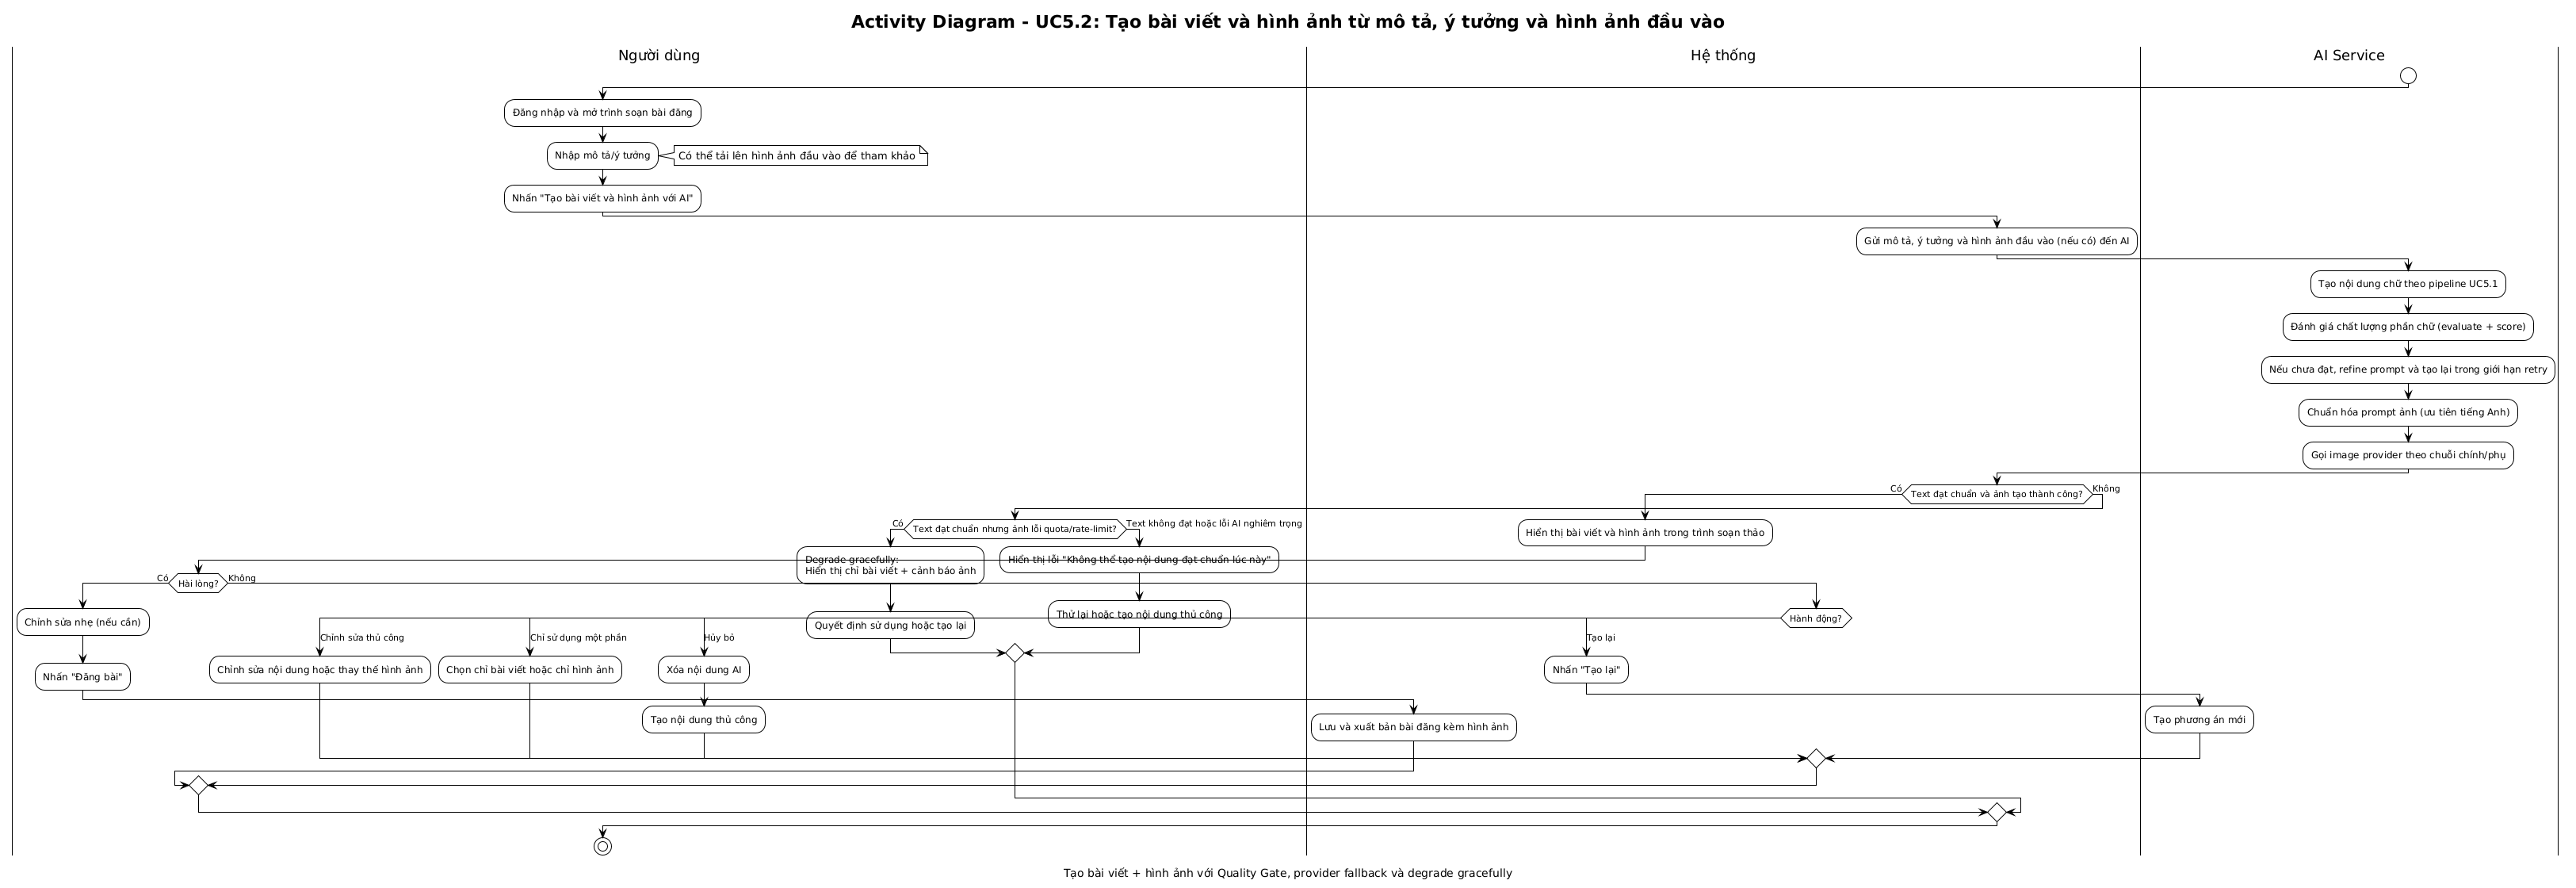
\includegraphics[width=\textwidth]{Images/Activity diagrams/AD-M5-UC5.2-GenerateImageText.png}
  \caption{Activity Diagram - Tạo bài viết và hình ảnh với đánh giá chất lượng riêng biệt (AD-M5-UC5.2-GenerateImageText)}
\end{figure}

\subsubsection{AD-M5-UC5.3-GenerateVideoImagesText}

Diagram này mô tả quy trình tạo nội dung đa phương thức (video + hình ảnh + bài viết) với pipeline đánh giá ba tầng.

\textbf{UC5.3 – Tạo video ngắn, hình ảnh và bài viết:} Người dùng nhập mô tả/ý tưởng và hình ảnh đầu vào (nếu có), nhấn ``Tạo video và nội dung đa phương thức với AI''. Hệ thống thực hiện quy trình sau:

\begin{enumerate}
    \item \textbf{Phân tích đầu vào}: Tương tự UC5.2, bổ sung xác định cấu trúc storyboard cho video (cảnh mở đầu, giới thiệu sản phẩm, highlight, CTA).
    \item \textbf{Xây dựng Prompt ba tầng}: Tạo prompt text $\rightarrow$ dùng text làm context tạo prompt image $\rightarrow$ dùng text + image làm context tạo prompt video. Prompt video bao gồm storyboard tự động, ràng buộc 15--30 giây, tỷ lệ 9:16 hoặc 1:1.
    \item \textbf{Gọi API tuần tự}: Gemini API cho text $\rightarrow$ Gemini API cho images (tối đa 3) $\rightarrow$ Google Veo 2 cho video.
    \item \textbf{Đánh giá chất lượng ba tầng}: Text (6 tiêu chí), Image (4 tiêu chí), Video (5 tiêu chí: Tính mạch lạc 0.25, Chất lượng hình ảnh 0.25, Độ dài phù hợp 0.15, Tính hấp dẫn 0.20, Nhất quán nội dung 0.15). Mỗi loại phải đạt $\geq$ 7.0/10.
    \item \textbf{Quyết định cải thiện có chọn lọc}: Chỉ tạo lại thành phần chưa đạt. Ví dụ: text và image đạt nhưng video chưa đạt $\rightarrow$ chỉ sửa prompt video và tạo lại video, giữ nguyên text và image. Tối đa 3 lần thử cho mỗi thành phần.
    \item \textbf{Hiển thị}: Video, hình ảnh và bài viết được hiển thị kèm điểm đánh giá từng loại. Người dùng có thể chỉnh sửa từng thành phần riêng biệt, tạo lại chỉ phần không hài lòng, hoặc thay thế bằng nội dung tự tạo.
\end{enumerate}

\begin{figure}[H]
  \centering
  \includegraphics[width=\textwidth]{Images/Activity diagrams/AD-M5-UC5.3-GenerateVideoImagesText.png}
  \caption{Activity Diagram - Tạo nội dung đa phương thức với pipeline đánh giá ba tầng (AD-M5-UC5.3-GenerateVideoImagesText)}
\end{figure}

\subsection{Module 6 – Post Scheduling}

Module này cho phép lên lịch đăng bài trong tương lai, quản lý bài đăng đã lên lịch (xem trước, chỉnh sửa, thay đổi thời gian, đăng ngay, xóa), và tự động xuất bản thông qua cron job.

\subsubsection{AD-M6-PostScheduling}

Diagram này mô tả quy trình lên lịch đăng bài và quản lý bài đăng đã lên lịch.

\textbf{UC6.1 – Lên lịch đăng bài:} Người dùng soạn bài đăng, chọn "Lên lịch" và chọn ngày/giờ xuất bản trong tương lai. Hệ thống kiểm tra thời gian hợp lệ, lưu bài đăng với trạng thái \textit{scheduled} và hiển thị thông báo. Nếu thời gian không hợp lệ, hệ thống báo lỗi.

\textbf{UC6.2 – Quản lý bài đăng đã lên lịch:} Người dùng xem danh sách bài viết chờ xuất bản. Người dùng có thể xem trước, chỉnh sửa nội dung/hình ảnh, thay đổi lịch đăng, đăng ngay, hoặc xóa bài viết. Mỗi hành động được cập nhật trong database ngay lập tức.

\textbf{Cron Job – Xuất bản tự động:} Cron job chạy định kỳ kiểm tra các bài viết có trạng thái \textit{scheduled} và thời gian xuất bản đã đến. Đối với mỗi bài viết đến hạn, cron job thay đổi trạng thái thành \textit{published}, xuất bản lên Feed và gửi thông báo đến tác giả.

\begin{figure}[H]
  \centering
  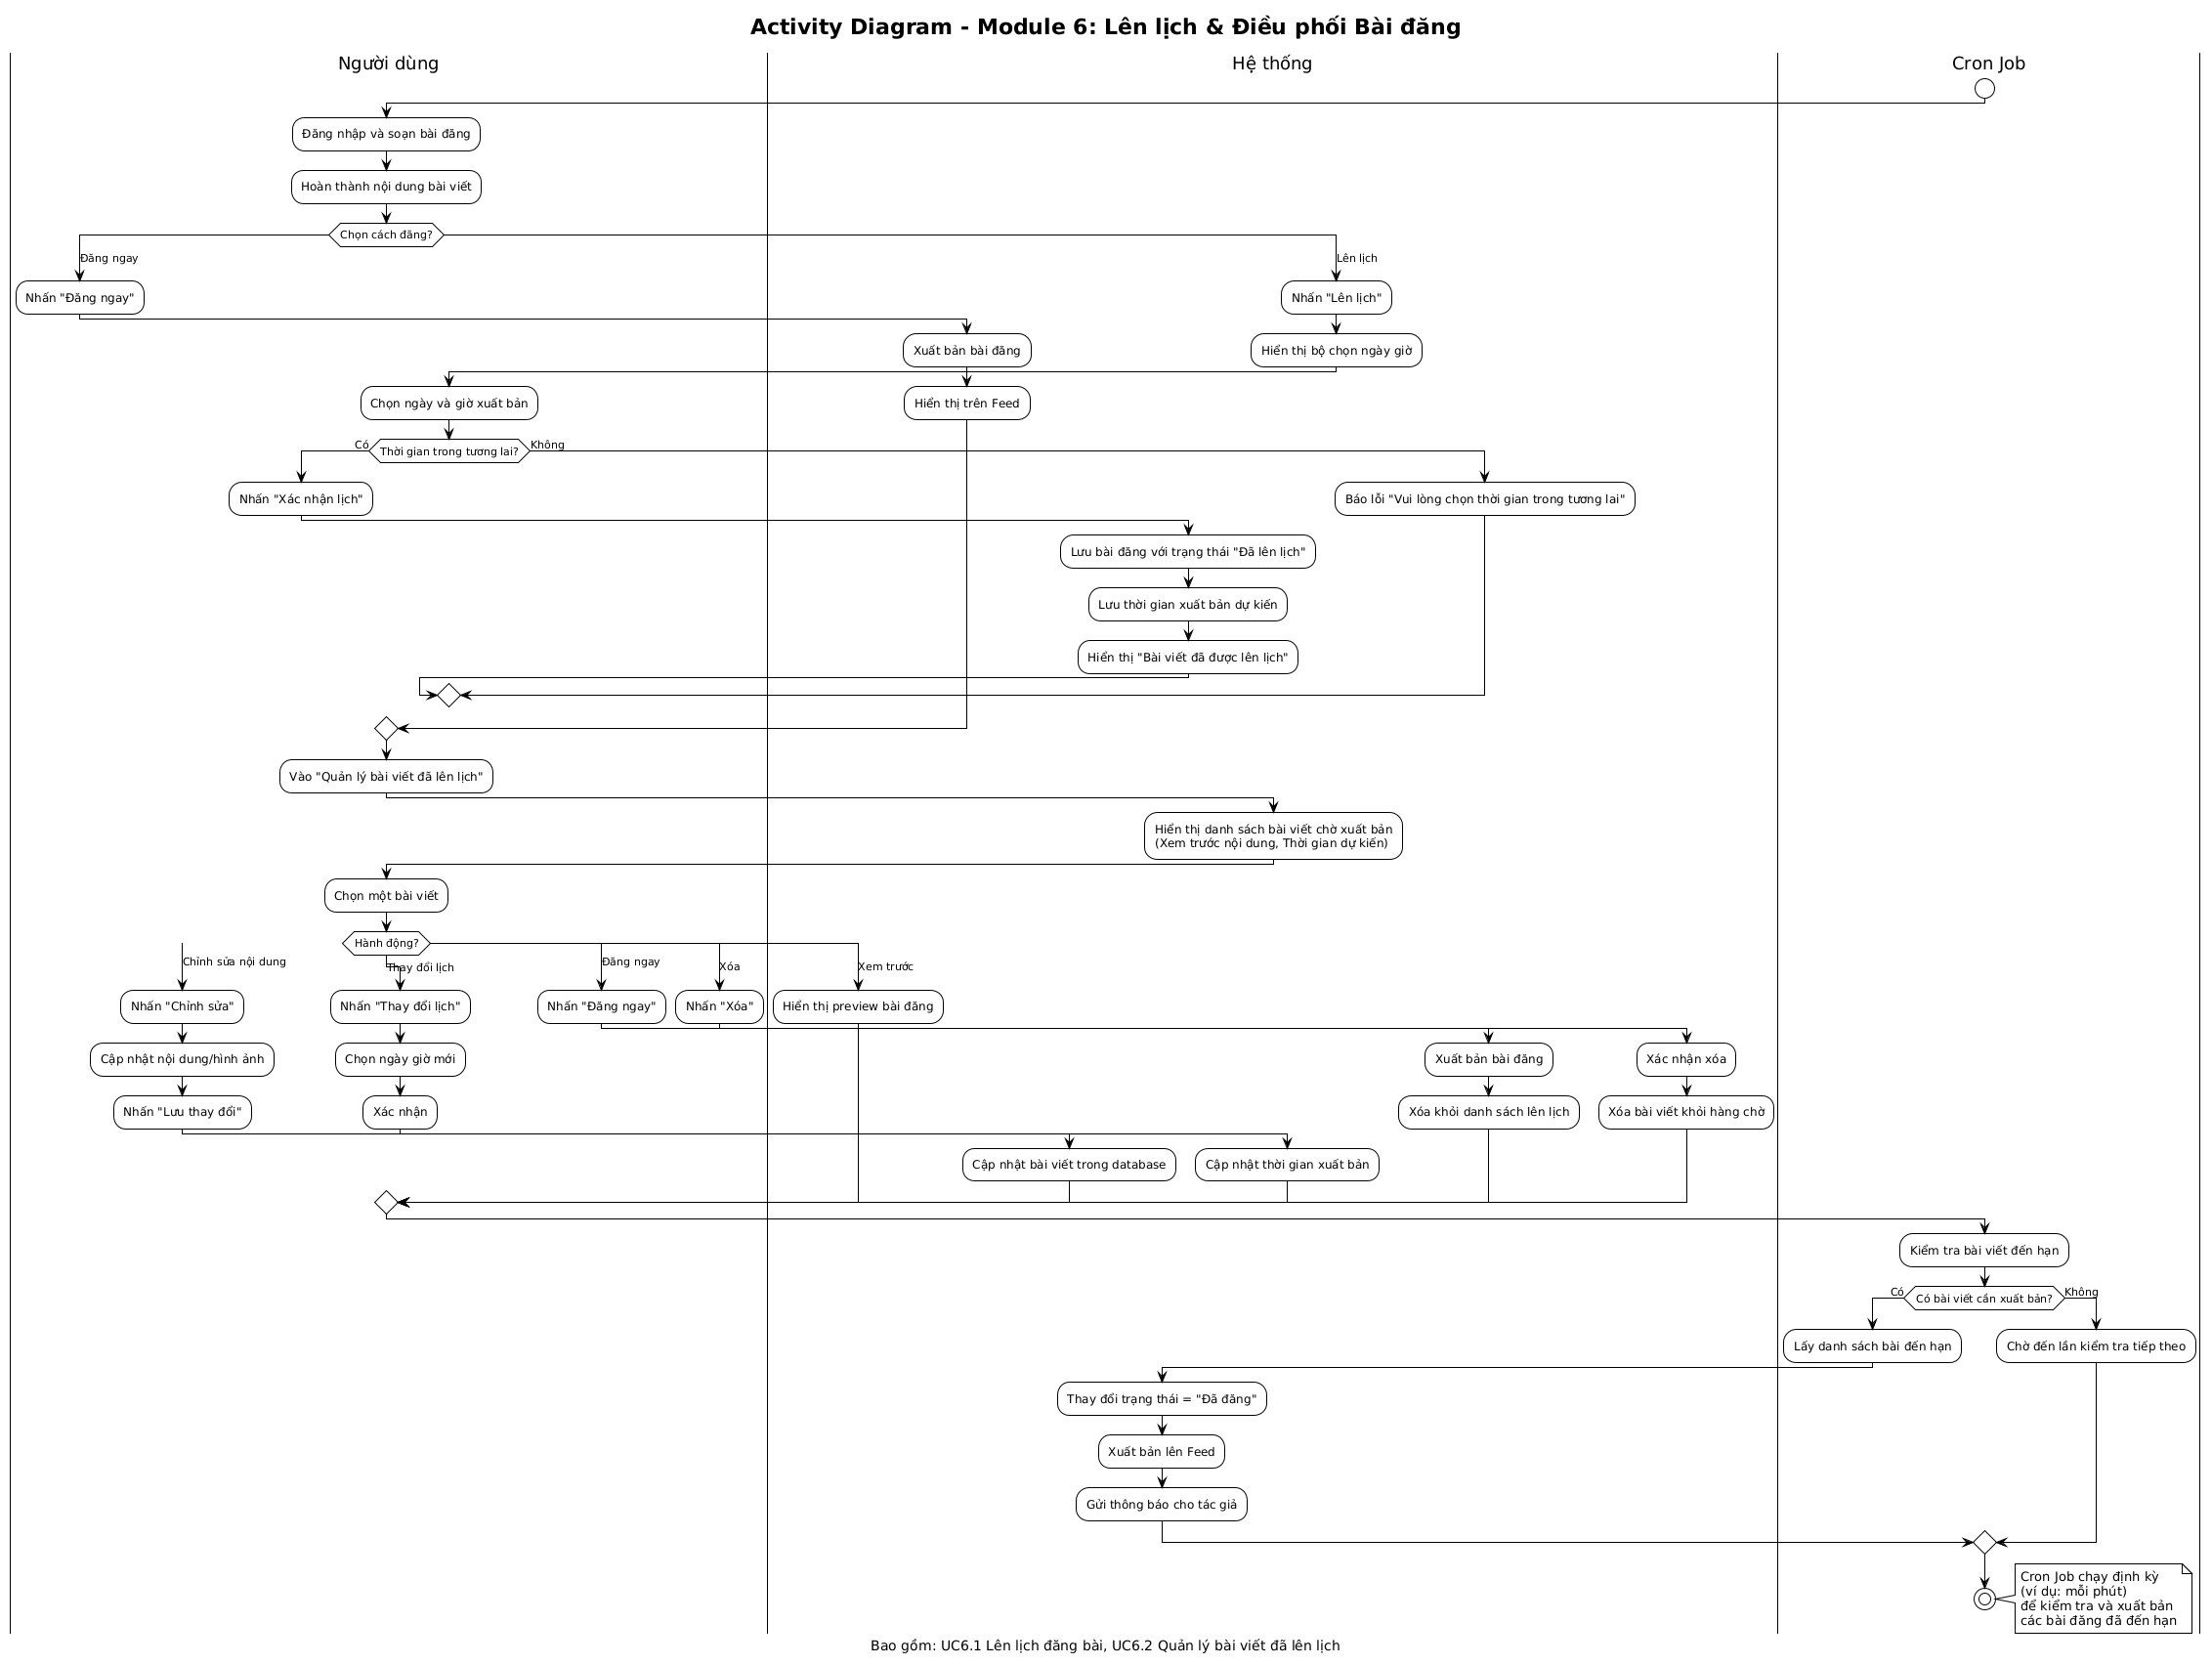
\includegraphics[width=\textwidth]{Images/Activity diagrams/AD-M6-PostScheduling.png}
  \caption{Activity Diagram - Lên lịch và Điều phối Bài đăng (AD-M6-PostScheduling)}
\end{figure}

\subsection{Module 7 – Notification}

Module này cung cấp hệ thống thông báo cho sự kiện tương tác xã hội (like, comment, follow, mention) và giao dịch (đơn hàng, hoàn tiền, đánh giá). Người dùng có thể quản lý thông báo (xem, đánh dấu đã đọc, xóa) và cấu hình nhận thông báo theo loại và kênh (web/email). Sử dụng WebSocket để gửi real-time khi online.

\subsubsection{AD-M7-NotificationSystem}

Diagram này mô tả toàn bộ hệ thống thông báo từ tạo, gửi, quản lý đến cấu hình.

\textbf{UC7.1 – Thông báo tương tác:} Khi A thực hiện tương tác với B (like, comment, follow, mention), hệ thống kiểm tra B có chặn A và cài đặt thông báo của B. Nếu cho phép, hệ thống tạo thông báo và lưu vào database. Nếu B đang online, gửi qua WebSocket ngay lập tức; nếu offline, lưu để hiển thị sau.

\textbf{UC7.2 – Thông báo giao dịch:} Hệ thống tạo và gửi thông báo cho các sự kiện: đơn hàng mới, xác nhận đơn, cập nhật trạng thái giao hàng, yêu cầu hoàn tiền, đánh giá mới. Tất cả thông báo được lưu vào database và gửi real-time nếu người nhận online và bật nhận loại thông báo này.

\textbf{UC7.3 – Quản lý thông báo:} Người dùng mở danh sách thông báo (sắp xếp theo thời gian, mới nhất ở trên). Người dùng có thể xem chi tiết, đánh dấu đã đọc (một hoặc tất cả), xóa một thông báo hoặc xóa tất cả (có xác nhận). Hệ thống cập nhật trạng thái và badge số thông báo chưa đọc.

\textbf{UC7.4 – Cài đặt thông báo:} Người dùng vào Cài đặt > Thông báo, bật/tắt từng loại thông báo (like, comment, follow, đơn hàng, đánh giá, tin nhắn, email) và chọn kênh nhận (web, email, hoặc cả hai). Hệ thống lưu cấu hình vào database và áp dụng ngay lập tức.

\begin{figure}[H]
  \centering
  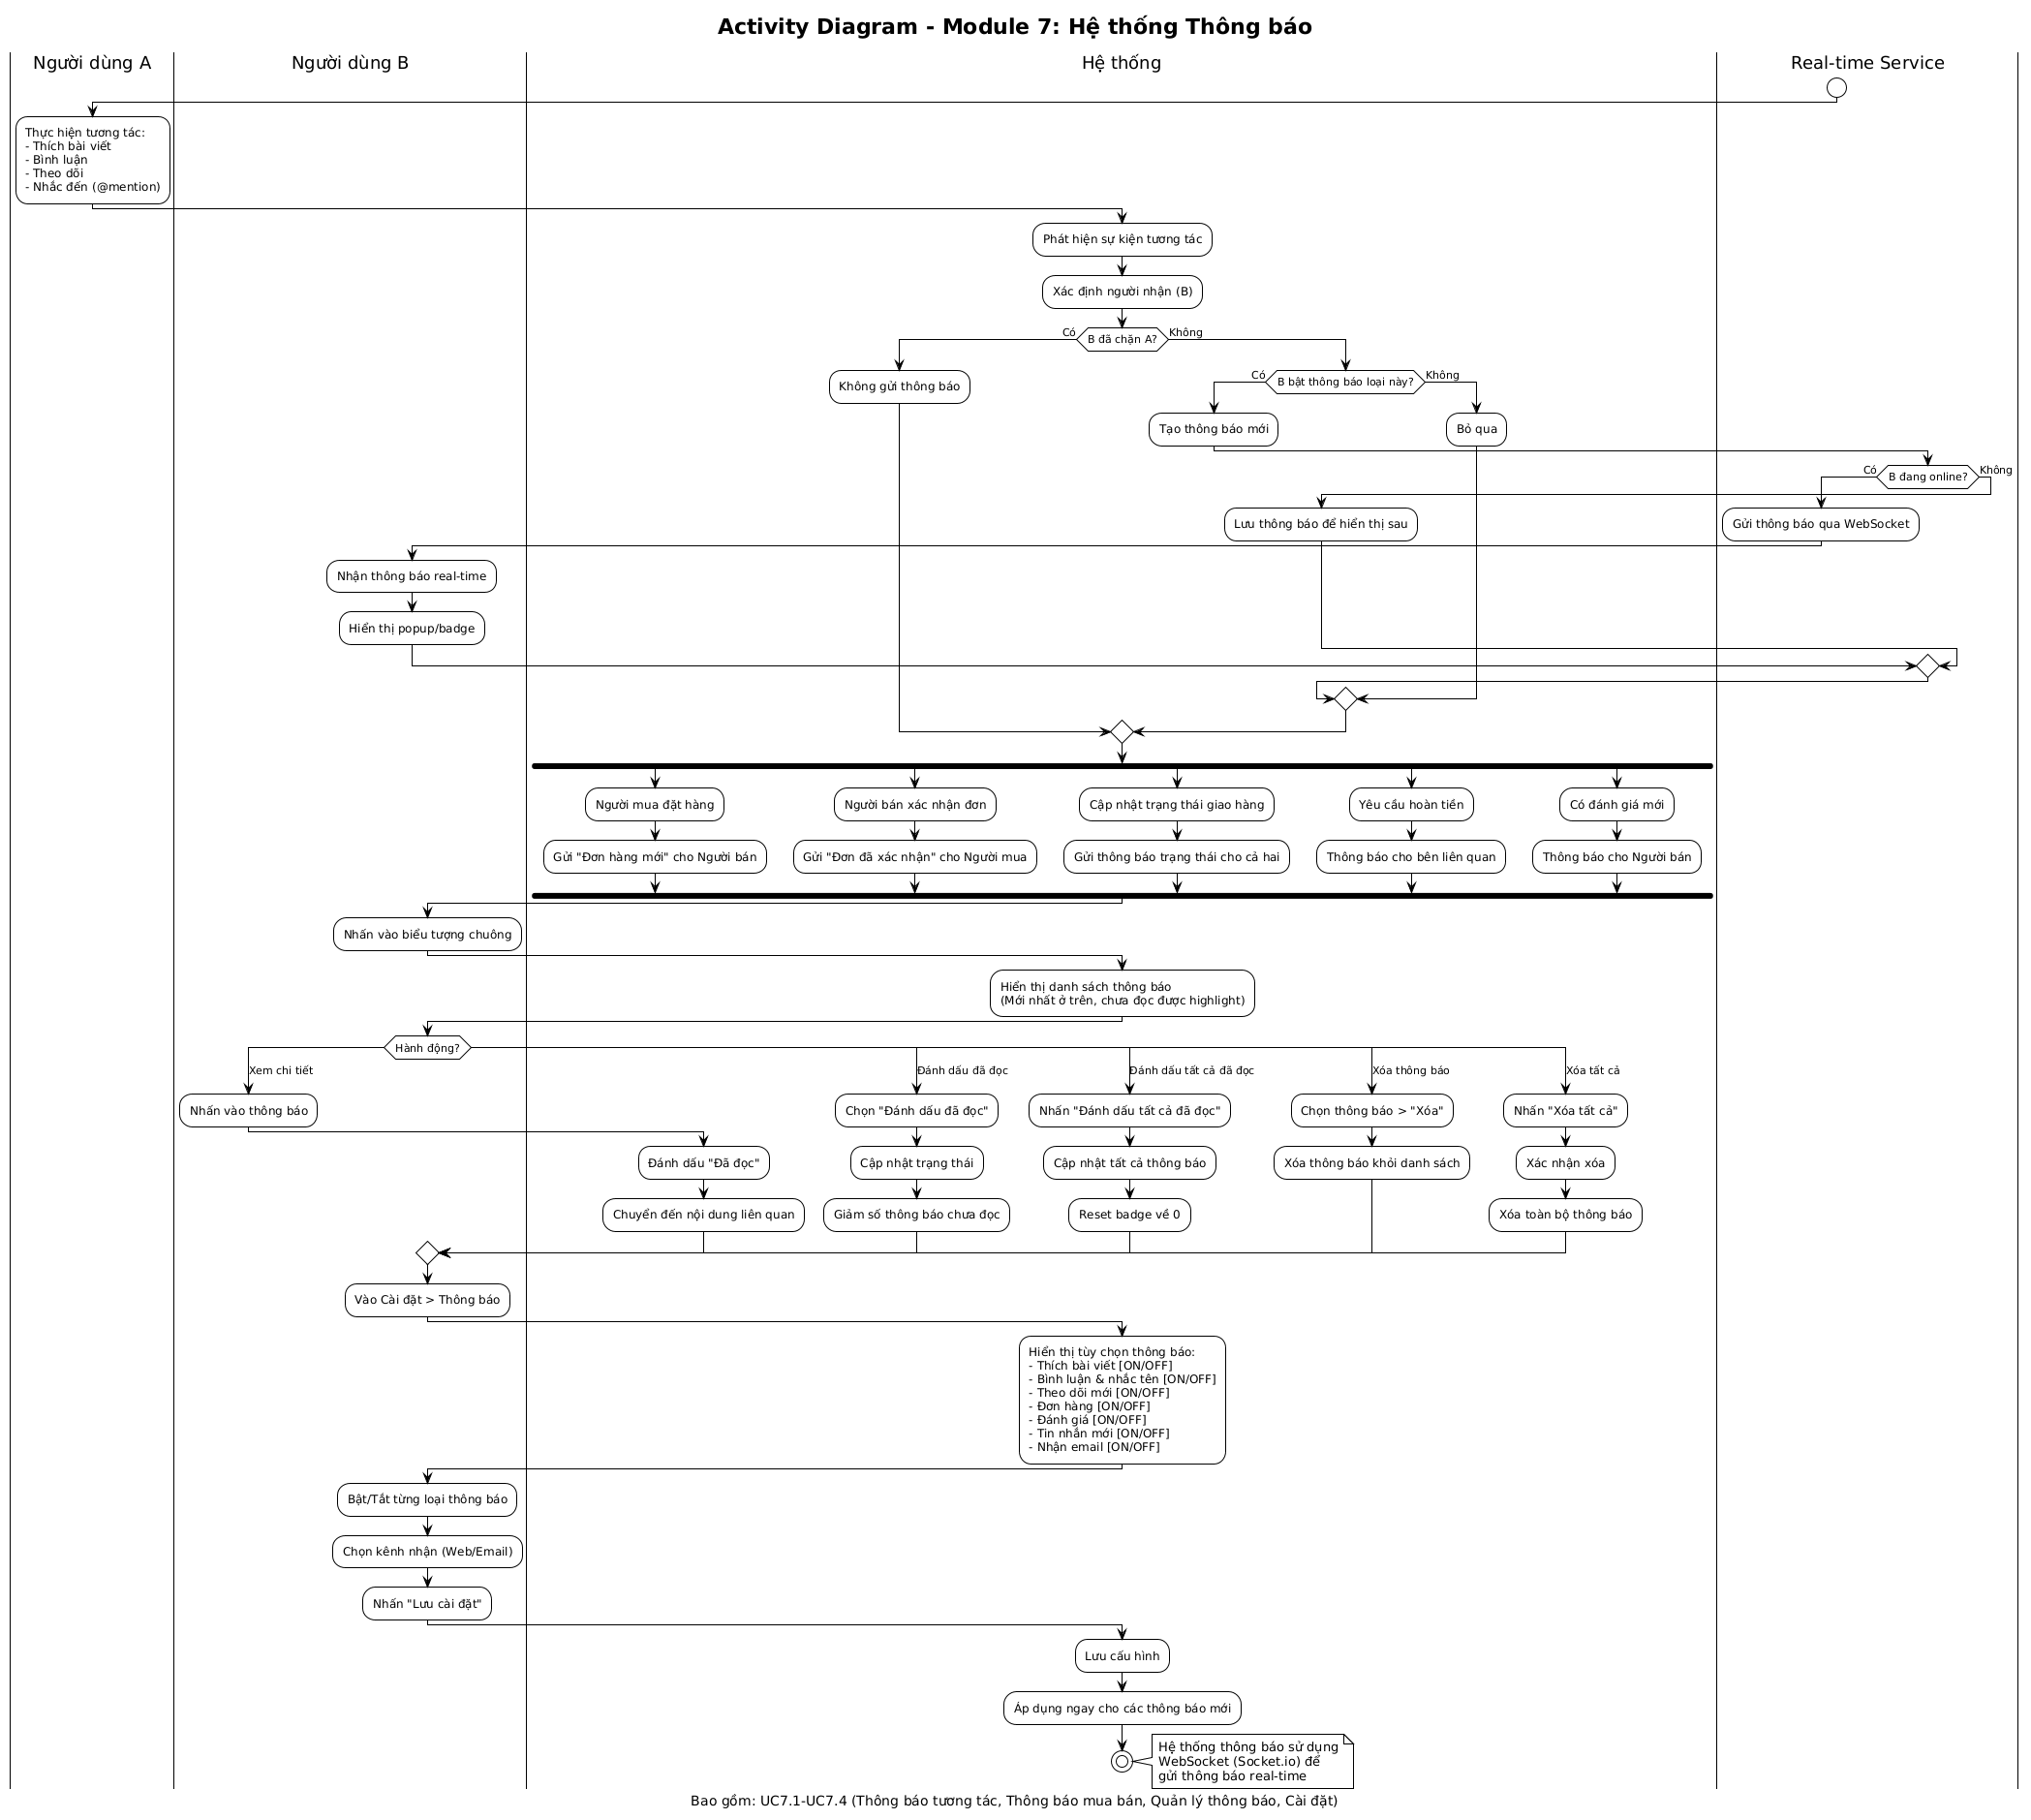
\includegraphics[width=\textwidth]{Images/Activity diagrams/AD-M7-NotificationSystem.png}
  \caption{Activity Diagram - Hệ thống Thông báo (AD-M7-NotificationSystem)}
\end{figure}
